\documentclass[math,code]{amznotes}
\setcounter{tocdepth}{2}  % Only show sections in the ToC
\usepackage[utf8]{inputenc}
\usepackage{amsmath}
\usepackage{amsfonts}
\usepackage{graphicx}
\usepackage{tikz}
\usepackage{etoolbox}
\usepackage{tabularx}
\usepackage{float} % Needed for [H] placement specifier
\usepackage{wrapfig} % Needed for wrapping figures
\usepackage{diagbox} % For diagonal split in table
\usepackage{booktabs} % For better table formatting
\usepackage{hyperref} % For hyper ref

\graphicspath{ {./images/} }
\geometry{
    a4paper,
    headheight = 1.5cm
}

\patchcmd{\chapter}{\thispagestyle{plain}}{\thispagestyle{fancy}}{}{}

\theoremstyle{remark}
\newtheorem*{claim}{Claim}
\newtheorem*{remark}{Remark}
\newtheorem{case}{Case}

\begin{document}
\fancyhead[L]{
    Quantitative Reasoning with Data
}
\fancyhead[R]{
    Lecture Notes
}
\tableofcontents

\chapter{Getting Data}
\section{Exploratory Data Analysis}
\begin{dfnbox}{Population}{dfn-population}
    A {\color{red} \textbf{population}} is the entire group (of individuals or objects) that we wish to know something about.
\end{dfnbox}
\begin{dfnbox}{Research Question}{dfn-research-question}
    A {\color{red} \textbf{research question}} is usually one that seeks to investigate some characteristic of a population.
\end{dfnbox}
Briefly speaking, we can classify \textbf{research questions} into the following categories
\begin{enumerate}
    \item To make an estimate about the population
    \item To test a claim about the population
    \item To compare two sub-populations / to investigate a relationship between two variables in the population
\end{enumerate}
\begin{dfnbox}{Exploratory Data Analysis (EDA)}{dfn-eda}
    {\color{red} \textbf{Exploratory Data Analysis (EDA)}} is a systematic process where we explore a data set and its variables and come up with \textbf{summary statistics} as well as \textbf{plots}. EDA is usually done \textbf{iteratively} until we find useful information that helps us answer the questions we have about the data set.
\end{dfnbox}
In general, the steps involved in EDA are:
\begin{enumerate}
    \item Generate \textbf{research questions} about the data.
    \item Search for answers to the research questions using data visualization tools. In the process of exploration, we could also perform data modeling. (e.g. regression analysis)
    \item We ask ourselves the following question: ``To what extent does the data we have, answer the questions we are interested in?''
    \item We refine our existing questions or generate new questions about the data before going back to data for further exploration.
\end{enumerate}

\section{Sampling}
The overall workflow for sampling is as follows (\textbf{This is very important}!)
\begin{enumerate}
    \item \textbf{Define Population of Interest}: Clearly identify the group you want to study.
    \item \textbf{Establish Sampling Frame}: Create or obtain a comprehensive list from which to select your sample.
    \item \textbf{Evaluate Sampling Frame Quality}: Check for issues such as:
    \begin{itemize}
        \item Coverage (does it include all population elements?)
        \item Relevance (does it contain extraneous units?)
        \item Duplication (are some units listed multiple times?)
        \item Clustering (are units grouped in a way that requires special sampling approaches?)
    \end{itemize}
    \item \textbf{Choose a Sampling Method and select sampling units}: Choose an appropriate technique (e.g., simple random, stratified, cluster sampling) based on your sampling frame characteristics.
    \item \textbf{Collect Data}: Gather the required \textbf{information} from your \textbf{selected sample}.
    \item \textbf{Calculate Estimates}: Use sample data to make inferences about the population parameters.
    \item \textbf{Assess Precision and Bias}: Evaluate the reliability of your estimates.
    \item \textbf{Make Inferences}: Draw conclusions about the population based on your sample data.
\end{enumerate}
\subsection{Basic Concepts and Definitions}
\begin{dfnbox}{Population of Interest}{dfn-population-of-interest}
    A {\color{red} \textbf{population of interest}} refers to a group in which we have interest in drawing conclusions in a study.
\end{dfnbox}
\begin{dfnbox}{Population Parameter}{dfn-population-parameter}
    A {\color{red} \textbf{population parameter}} is a \textbf{numerical} fact about a population.
\end{dfnbox}
\begin{exbox}{Example of Population Parameters and Population}{example-of-population-parameters-and-population}
    \raggedright % Prevent justification issues
    The following are some examples of a population and an associated population parameter.
    \begin{enumerate}
        \item The \underline{average height} (population parameter) of \underline{all primary six students in a particular primary school} (population).
        \item The \underline{median number of modules taken} (population parameter) by \underline{all first-year undergraduates in a University} (population).
        \item The \underline{standard deviation of the number of hours spent on mobile games} (population parameter) by \underline{pre-schoolers aged 4 to 6 in Singapore} (population).
    \end{enumerate}
\end{exbox}
\begin{dfnbox}{Census}{dfn-census}
    A {\color{red} \textbf{census}} is a \textbf{method of data collection} from everyone. It attempts to reach out to the entire population of interest.\footnote{Note that since a census does
not involve sampling, the notion of sampling frame is not applicable in that context.}
\end{dfnbox}
Some disadvantages of conducting a census are as follows:
\begin{enumerate}
    \item Conducting a census is often prohibitively expensive.
    \item Some studies require timely data, but censuses typically take a long time to complete.
    \item Even when attempted, a census may not achieve a 100\% response rate.
\end{enumerate}
\begin{dfnbox}{Sampling}{dfn-sampling}
    As contrast to \textbf{census}, if we don't reach out to everyone from the entire population of interest, we only select part of them using the sampling methods we will introduce later, this \textbf{method of data collection} is called {\color{red} \textbf{sampling}}.
\end{dfnbox}
In \textbf{Sampling}, we have the following important three concepts:
\begin{enumerate}
    \item \textbf{Sampling Frame}\footnote{The \textbf{sampling frame} provides \textbf{a list of samples} we can select our sample from.}: A \textbf{sampling frame} is the list from which the \textbf{sample} was obtained.
    \item \textbf{Sample}\footnote{Doing so is because it is usually not feasible to gather information from every member of the population}: A \textbf{sample} is a \textbf{proportion of the population} selected in the study. It's fundamental element is called \textbf{sampling unit} and it is selected from the \textbf{sampling frame}.
    \item \textbf{Estimate}: An \textbf{Estimate} is an inference about the \textbf{population parameter} based on the information obtained from a \textbf{sample}.
\end{enumerate}

In EDA, the most important question is whether the sample obtained from such a sampling frame is still \textbf{able to tell us something about the population parameter}. Regarding this, the following are some important characteristics of \textbf{sampling frame}:
\begin{enumerate}
    \item Does the sampling frame include \textbf{all available sampling units}\footnote{Sampling units are the individual elements or entities that are selected from a population when conducting a survey or research study.} from the population?
    \item Does the sampling frame contain \textbf{irrelevant} or \textbf{extraneous} sampling units from another population?
    \item Does the sampling frame contain \textbf{duplicated} sampling units?
    \item Does the sampling frame contain sampling units in \textbf{clusters}?
\end{enumerate}
In our sampling frame, we are more interested in the \textbf{generalisability}, which is the ability to generalise the findings from a sample to the population. And the requirement is that the \textbf{sampling frame must be equal to or greater than the population of interest}.\footnote{This means that the sampling frame should include \textbf{every sampling unit} from the population of interest.}

\textbf{Population of Interest vs. Sampling Frame vs. Sample}
\begin{enumerate}
    \item \textbf{Population of Interest}
    \begin{itemize}
        \item The complete set of individuals or units you want to study and make conclusions about
        \item Example: All people who drink coffee in Singapore
    \end{itemize}
    
    \item \textbf{Sampling Frame}
    \begin{itemize}
        \item The operational list or source from which you actually select your sample
        \item It's your practical way to access the population
        \item Example: A customer database from coffee shops, a residential directory, or registered participants in a consumer survey who indicated they drink coffee
    \end{itemize}
    
    \item \textbf{Sample}
    \begin{itemize}
        \item The subset of units actually selected from the sampling frame for data collection
        \item These are the specific individuals or units you'll gather information from
        \item Example: The 500 coffee drinkers you ultimately survey or interview
    \end{itemize}
\end{enumerate}
The relationships between them:
\begin{itemize}
    \item Ideally, your sampling frame would perfectly match your population of interest, but this rarely happens in practice
    \item Your \textbf{sample is drawn directly from your sampling frame}, not from the theoretical population
    \item Any limitations in your sampling frame (like missing certain types of coffee drinkers) will affect how well your sample represents your population of interest
\end{itemize}
\subsection{Bias}
\textbf{Bias} refers to systematic errors that skew sample data, preventing it from accurately representing the population and leading to unreliable conclusions. One consequence is that, even if our \textbf{sampling frame} covers the entire population of interest, our findings from the sample \textbf{may not always be generalisable} to the population. There are \textbf{two} major kinds of biases.
\begin{enumerate}
    \item \textbf{Selection Bias}: Occurs when the researcher’s \textbf{biased selection of units} -- due to an imperfect sampling frame or non-probability sampling -- excludes certain units, preventing the sample from representing the population accurately.
    \item \textbf{Non-response Bias}: Arises from \textbf{participants’ non-participation or non-disclosure}, excluding their information due to reasons like inconvenience or sensitivity, regardless of the sampling method used.
\end{enumerate}
\begin{notebox}
    \begin{remark}
        The \textbf{bias} will affect the construction of our \textbf{sampling frame}, and since our \textbf{sample units} are chosen from the sampling frame to form the \textbf{sample we want to gather information from}, so it will affect our \textbf{generalisability} from sample to population.
    \end{remark}
\end{notebox}

\subsection{Probability Sampling}
\begin{dfnbox}{dfn-probability-sampling}
    \textbf{Probability sampling}  is a sampling scheme such that the selection process is done via a known randomised\footnote{The randomized mechanism is important as it introduces an element of chance in the selection process so as to \textbf{eliminate biases}.} mechanism.\footnote{ It is important that every unit in the sampling frame has a \textbf{known non-zero probability} of being selected but the probability of being selected does not have to be same for all the units.}
\end{dfnbox}
We will introduce four main types of probability sampling methods:
\subsubsection{Simple Random Sampling}
\textbf{S}imple \textbf{R}andom \textbf{S}ampling, or SRS, is a method where every possible group of $n$ units from the population has an equal chance of being selected. For example, to choose 5 students from a class of 30, assign each student a number from 1 to 30 and use a \textbf{random number generator} to pick 5 distinct numbers.
\begin{notebox}
    \begin{enumerate}
        \item SRS is usually achieved by using a \textbf{random number generator}. However, one \textbf{shortcoming} for SRS is that it can possibly subjected to \textbf{non-response} from the units that are sampled.
        \item SRS needs to know the number \textbf{whole sampling unit in the population}! Otherwise, you can't ensure that you can't ensure that every group of $n$ has an equal probability of selection. Alternatively speaking, when you use your calculator, like CASIO 991 to implement a random number generator, you need to specify the range of your numbers (you total sampling unit).
    \end{enumerate}
\end{notebox}
\subsubsection{Systematic Sampling}
Systematic sampling is a method of selecting units from a \textbf{list}\footnote{the ``list'' refers to the sampling frame, which is a complete list of all units in the population that you can sample from.} by applying a selection interval $k$ and a \textbf{random starting point} from the \textbf{first interval}. To carry out systematic sampling:
\begin{enumerate}
    \item Suppose we know how many sampling units there are in the population (denoted by $p$)
    \item We decide how big we want our sample to be (denoted by $n$). This means that we will select one unit from every $k=\frac{p}{n}$ units;
    \item From 1 to $k=\frac{p}{n}$, select a number \textbf{at random}, say $r$
    \item With this, the sample will consist of the following units from the list:
    \begin{displaymath}
        r, r+k, r+2k, \cdots,r+(n-1)
    \end{displaymath}
\end{enumerate}
However, it is \textbf{often} that we do not know the number of sampling units $p$ in the population. In such a situation, systematic sampling can still be done by \textbf{deciding on the selection interval} $k$ and randomly selecting a unit from the first $k$ units and then subsequently every $k$th unit will be sampled. For example, if $k = 10$, we can sample the $5^\text{th}, 15^\text{th}, 25^\text{th}$ units and so on.
\begin{notebox}
    \begin{enumerate}
        \item Compared to SRS, systematic sampling doesn't need to know the whole sampling units in the sampling frame.
        \item The shortcome is that, if the \textbf{list}, or \textbf{sampling frame}, is \textbf{not random}, but instead contains some inherent grouping or ordering of the units, then the sample generated by \textbf{systematic sampling} may not be \textbf{representative} of the population.
    \end{enumerate}
\end{notebox}

\subsubsection{Stratified Sampling}
Stratified Sampling is a sampling method that combines the idea of ``classification'' and ``randomization'' and it is achieved as follows:
\begin{enumerate}
    \item The sampling frame is divided into groups called \textbf{strata}. Each \textbf{stratum} is \textbf{similar in that they share similar characteristics} but the size of each stratum does not necessarily have to be the same.
    \item SRS is then applied to each stratum to generate the whole sample.
\end{enumerate}
\begin{notebox}
    \begin{enumerate}
        \item Because of the property of \textbf{stratum}, which is within each stratum, the sample units must share similar characteristic, it is sometimes hard to form such stratum.
    \end{enumerate}
\end{notebox}

\subsubsection{Cluster Sampling}
It is similar to Stratified Sampling, but the difference lies in \textbf{how the whole sampling frame is classified}
\begin{enumerate}
    \item Divide the sampling frame into \textbf{clusters}, where \textbf{clusters} doesn't have any requirements for its inner sampling units, thus ensuring the \textbf{inner diversity}
    \item Use SRS to select \textbf{a fixed number of clusters}\footnote{Now sampling units within each cluster here}.
    \item All the sampling units from the selected clusters are then included in the overall sample.
\end{enumerate}

Table \ref{tab:chapter1-comparison-of-sampling-plans} summarizes the advantages and disadvantages for the four probability sampling methods we have learned
\begin{table}[h]
\centering
\begin{tabular}{|>{\raggedright\arraybackslash}p{4cm}|>{\raggedright\arraybackslash}p{5cm}|>{\raggedright\arraybackslash}p{6cm}|}
\hline
\textbf{Sampling Plan} & \textbf{Advantages} & \textbf{Disadvantages} \\
\hline
Simple Random Sampling & Good representation of the population & Time-consuming; accessibility of information and sampling frame \\
\hline
Systematic Sampling & Simple selection process as opposed to simple random sampling & Potentially under-representing the population \\
\hline
Stratified Sampling & Good representation of the sample by stratum & Require sampling frame and criteria for classification of the population into stratum \\
\hline
Cluster Sampling & Less time-consuming and less costly & Require clusters to be reasonably heterogeneous\footnote{``heterogeneous'' means that \textbf{each cluster} should ideally \textbf{reflect the diversity of the entire population}.} and not have cluster-specific characteristics \\
\hline
\end{tabular}
\caption{Comparison of Sampling Plans}
    \label{tab:chapter1-comparison-of-sampling-plans}
\end{table}

\subsection{Non-probability Sampling}
\begin{dfnbox}{dfn-non-probability-samping}
    A \textbf{non-probabilty sampling} method is when the selection of units is \textbf{not done by randomisation}.
\end{dfnbox}
\subsubsection{Convenience Sampling}
Convenience sampling is when a researcher chooses the sampling units to form a sample among those that are most easily available to participate in the study.
\subsubsection{Volunteer Sampling}
Volunteer sampling is when the sampling units \textbf{volunteer} themselves into a sample.

\section{Variables and Summary Statistics}
\subsection{Variables}
Let's kick start this part by introducing some concepts
\begin{enumerate}
    \item A \textbf{variable} is an attribute that can be measured or labelled.
    \item A \textbf{data set} is a collection of \textbf{individuals} and \textbf{variables pertaining to the individuals}. Individuals can refer to either objects or people.
\end{enumerate}
In a \hyperref[dfn:dfn-research-question]{research question} where we are examining relationships between variables, there is usually a distinction between which are \textbf{independent variables} and which are \textbf{dependent variables}.
\begin{notebox}
    \begin{remark}
        It is important to note that the dependent variable is \textbf{hypothesised to change} when the independent variable is manipulated. It does not mean that the dependent variable \textbf{must} change.
    \end{remark}
\end{notebox}
\subsubsection{Types of Variables}
\begin{enumerate}
    \item \textbf{Categorical Variable}: Variables that take on categories or label values. These categories or labels are \textbf{mutually exclusive}.
    \begin{itemize}
        \item \textbf{Ordinal Variable}: A categorical variable where there is some natural ordering and numbers can be used to represent the ordering.
        \item \textbf{Nominal Variable}: A categorical variable where there is no intrinsic ordering
    \end{itemize}
    \item \textbf{Numerical Variable}: Variables that take on numerical values and we are able to \textbf{meaningfully perform arithmetic operations} like adding and taking average.
    \begin{itemize}
        \item \textbf{Discrete Variable}: A numerical variable where there are gaps in the set of possible numbers taken on by the variable. For example, the number of students can only be \textbf{integer}, cannot have fraction.
        \item \textbf{Continuous Variable}: A numerical variable that can take on all possible numerical values in a given range or interval. For example, the height of a student can be any number, not restricted to integer only.
    \end{itemize}
\end{enumerate}

\subsection{Summary Statistics}
Summary Statistics can be divided into two parts
\begin{enumerate}
    \item Those that measure \textbf{central tendencies} of the data, like \textbf{mean, median} and \textbf{mode}
    \item Those that measure the \textbf{level of dispersion (or spread)} of the data, like \textbf{standard deviation} and \textbf{interquartile range}.
\end{enumerate}
\subsubsection{Measure Central Tendencies}
\textbf{Mean} \\
The mean is simply the average value of a numerical variable $x$. We denote the mean of $x$ by $\bar{x}$ and the formula to compute $\bar{x}$ is
\begin{displaymath}
    \bar{x} = \frac{x_1+x_2+\cdots x_n}{n}=\frac{\Sigma_{i=1}^n~x_i}{n}
\end{displaymath}
There are some properties of the \textbf{mean} of a variable
\begin{enumerate}
    \item Even if we don't know each of the individual value, we can still calculate the sum, given the value of $\bar{x}$ and the number of data points $n$, by using $\text{sum}=\bar{x}\times n$
    \item Adding a constant value $c$ to all the data points changes the mean by that constant value. For example, if we add a constant $c$ to each of the data point, the new mean will be $\bar{x}+c$
    \item Multiplying a constant value of $c$ to all the data points will result in the new mean being changed by the same factor of $c$. For example, if we multiply a constant $c$ to each of the data point, the new mean will be $c\times\bar{x}$
\end{enumerate}

\textbf{Median}\\
The median is simply the middle value of the variable after arranging the values of the data set in ascending or descending order. \hypertarget{chapter1-median-meaning}{The meaning of \textbf{median} is that there are 50\% data points which are below the median, and correspondingly, there are 50\% data points which are above the median.}
\begin{notebox}
    \begin{remark}
        If there are two middle values (when there are an even number of data points), we will take the \textbf{average} of the two middle values as the median.
    \end{remark}
\end{notebox}
There are some properties of \textbf{median} also
\begin{enumerate}
    \item Adding a constant value $c$ to all data points will result in the new median being \textbf{added} by the constant $c$.
    \item Multiplying a constant value $c$ to all data points will result in the new median being \textbf{multiplied} by the constant $c$.
\end{enumerate}

\textbf{Mode}\\
The mode is a variable that appears \textbf{most often} in data.
\begin{notebox}
    \begin{remark}
        Mode is applicable to both \textbf{numerical} and \textbf{categorical} variables.
    \end{remark}
\end{notebox}

\subsubsection{Measure Spread}
\textbf{Standard Deviation} \\
Standard deviation is one of the ways to measure the \textbf{spread} of the data about the \textbf{mean} (denoted by $\bar{x})$. It can be computed as follows
\begin{align*}
    \text{Sample Variance, Var}&=\frac{(x_1-\bar{x})^2+(x_2-\bar{x})^2+\cdots+(x_n-\bar{x})^2}{n-1} \\
    \text{Standard Deviation, }s_x&=\sqrt{\text{Var}}
\end{align*}
\begin{notebox}
    \begin{remark}
        The reason for the denominator to be $n-1$ not $n$ is beyond the scope of this course.
    \end{remark}
\end{notebox}
There are some properties of the \textbf{standard deviation} of the data
\begin{enumerate}
    \item The standard deviation $s_x$ is always \textbf{non-negative}. Only when all the data points are of the same value then $s_x=0$
    \item The standard deviation shares \textbf{the same unit} as the numerical variable $x$.
    \item Adding a constant $c$ to all data points \textbf{doesn't change} the standard deviation.
    \item Multiplying a constant $c$ to all data points results in the standard deviation being multiplied by $|c|$, which is the absolute value of $c$.
\end{enumerate}
\textbf{Interquartile Range (IQR)} \\
As we have seen above about the \hyperlink{chapter1-median-meaning}{meaning of median}, median is also called the $50^{th}$ percentile of the data values. Similarly, we have 
\begin{enumerate}
    \item \textbf{The first quartile}, denoted by $Q_1$, is the $25^{th}$ percentile of the data values.
    \item \textbf{The third quartile}, denoted by $Q_3$, is the $75^{th}$ percentile of the data values.
    \item \textbf{The Interquartile Range (IQR)}, which is $Q_3-Q_1$
\end{enumerate}
Similarly, there are some properties about the IQR
\begin{enumerate}
    \item IQR is \textbf{non-negative}
    \item Adding a constant $c$ to all data points \textbf{doesn't change} the IQR.
    \item Multiplying a constant $c$ to all data points results in the IQR being multiplied by $c$
\end{enumerate}
To find/calculate the $Q_1$ and $Q_3$ of a variable, given that the number of data points is $n$, we can use
\begin{enumerate}
    \item \textbf{Find the median} of the total $n$ data points.
    \item \textbf{Divide the data into upper half and lower half} according to the median
    \begin{itemize}
        \item If $n$ is \textbf{even}, just divide normally
        \item If $n$ is \textbf{odd}, \textbf{exclude} the median from the upper half
    \end{itemize}
    \item \textbf{Find} $Q_1$ and $Q_3$
    \begin{itemize}
        \item $Q_1$ is the median of the lower half.
        \item $Q_3$ is the median of the upper half.
    \end{itemize}
\end{enumerate}

\chapter{Categorical Data Analysis}
\section{Rates}
\begin{dfnbox}{Rates}{def-rates}
    In categorical data analysis, a {\color{red} \textbf{rate}} (also called a proportion or relative frequency) quantifies how frequently a specific category occurs within a dataset. It is calculated as the ratio of the number of observations in a \textbf{given category} (a.k.a \textbf{target}) to the \textbf{total} number of observations (a.k.a \textbf{population}). {\color{red} \textbf{Rates}} are typically expressed as a fraction (between 0 and 1) or a percentage (between 0\% and 100\%), providing a standardized measure of prevalence or likelihood for that category.
\end{dfnbox}
\begin{notebox}
    \begin{remark}
        Based on the fact the \textbf{rate} are always between 0 and 1 (or 0\% and 100\%), we can intuitively see that \textbf{rate} can be used as a fair comparison when group sizes are unequal. This idea is known as ``changing from absolute numbers to percentage''.
    \end{remark}
\end{notebox}
\begin{exbox}{One Variable Rate Example}{example-rate-one-variable}
    A survey asks 500 people, ``Do you prefer tea or coffee?'' Of the respondents, 200 select ``Tea'' and 300 select ``Coffee''.
    \begin{align*}
        \text{rate(tea)}=\frac{200}{500}=0.4\text{(or 40\%)} \\
        \text{rate(coffee)}=\frac{300}{500}=0.6\text{(or 60\%)}
    \end{align*}
\end{exbox}
\begin{notebox}
    \begin{remark}
        For every \textbf{rate} problem, we need to find out what is our \textbf{population}, this is become the denominator. And what is our \textbf{target}, this will become our nominator.
    \end{remark}
\end{notebox}
Before we go deeper into the three different kinds of rates, let's give out the following table,
\begin{table}[h]
    \centering
    \begin{tabular}{|c|c|c|c|}
        \hline
        \diagbox{Treatment}{Outcome} & Success & Failure & Row Total \\ 
        \hline
        X & 542 & 158 & 700 \\ 
        \hline
        Y & 289 & 61 & 350 \\ 
        \hline
        Column Total & 831 & 219 & 1050 \\ 
        \hline
    \end{tabular}
    \caption{Kidney Problem}
    \label{tab:table-kidney-1}
\end{table}
\begin{notebox}
    \begin{remark}
        This table is known as a \textbf{$2\times 2$ contingency table}. And the dependent variable \textit{Outcome} is placed on the columns on the table while the independent variable \textit{Treatment} is placed on the rows.
        
    \end{remark}
\end{notebox}

\subsection{Marginal Rate}
\begin{dfnbox}{Marginal Rate}{def-marginal-rate}
    {\color{red} \textbf{Marginal rate}}, as its name suggests, are calculated by two \textbf{marginal} numbers in the table.
\end{dfnbox}
\begin{exbox}{Marginal rate Example}{example-marginal-rate}
    In the table \ref{tab:table-kidney-1} given above, suppose we want to know what proportion of total number of patients were given treatment Y and the proportion of total number of patients were given \textbf{success} treatment. \\
    \textbf{Solution:} This problem is actually a \textbf{marginal rate} problem. And the two marginal data we need are labeled as red as follows:
    \begin{figure}[H]
        \centering
        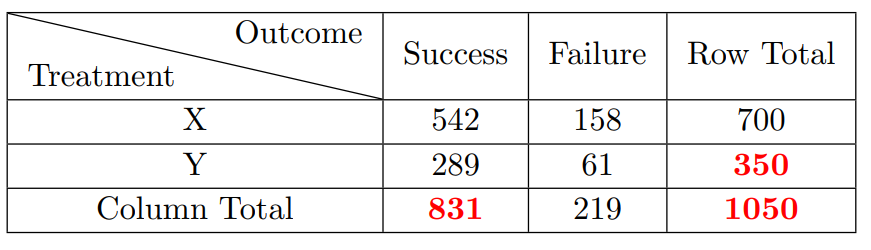
\includegraphics[width=0.75\linewidth]{images/chapter2-marginal-rate.png}
        \caption{Kidney Problem (Marginal rate)}
        \label{fig:table-kidney-2}
    \end{figure}
    So, we can calculate our rate(Y)\footnote{``Y'' represents the patients who are given treatment Y} as follows:
    \begin{displaymath}
        \text{rate(Y)}=\frac{350}{1050}=33\frac{1}{3}\%
    \end{displaymath}
    Similarly, rate(X)\footnote{``X'' represents the patients who are given successful treatments} is also a marginal rate and will be
    \begin{displaymath}
        \text{rate(X)}=\frac{831}{1050}=66\frac{2}{3}\%
    \end{displaymath}
\end{exbox}

\subsection{Conditional Rate}
\begin{dfnbox}{Conditional rate}{dfn-conditional-rate}
    {\color{red} \textbf{Conditional rate}}, as its name suggests, must set a \textbf{condition} for the calculation of the rate.
\end{dfnbox}
\begin{exbox}{Conditional rate example}{example-conditional-rate}
    For example, with Table \ref{tab:table-kidney-1}, if we want to know \textit{Among those patients given treatment X, what proportion were successful?}. \\ 
    \textbf{Solution:} This is a \textbf{conditional rate} problem. The condition specifies our \textbf{population} (X) to be 700. From the question, our \textbf{target} (Success given/under condition X) is 542. Thus, the conditional rate rate(Success | X) is calculated by:
    \begin{displaymath}
        \text{rate(Success | X)}=\frac{542}{700}=0.774=77.4\%
    \end{displaymath}
\end{exbox}
\begin{notebox}
    \begin{remark}
        The notation rate(target | condition), is used often for the \textbf{conditional rate}. It basically means the \textbf{rate} (\textit{target} given/under the \textit{condition}), which implicitly specifies the \textbf{population} to be the data that satisfies the condition.
    \end{remark}
\end{notebox}
\subsubsection{Application of conditional rate}
One real-world application of the conditional rate is that it can give us information about the \textbf{association} between two variables. We will see more about this later in this chapter.

But for now, with our example in table \ref{tab:table-kidney-1}, since $\text{rate(Success | Y)}=\frac{289}{350}=82.6\%$ is higher than $\text{rate(Success | X)}=\frac{542}{700}=77.4\%$, we can intuitively find out that Treatment Y is more effective than Treatment X.

\subsection{Joint Rate}
\begin{dfnbox}{Joint-Rate}{dfn-joint-rate}
    {\color{red} \textbf{Joint Rate}} means that our \textbf{target} is \textbf{not a marginal data} and our \textbf{population} is the \textbf{whole population} (the right-bottom corner of the table \ref{tab:table-kidney-1}).
\end{dfnbox}
\begin{notebox}
    \begin{remark}
        A joint rate problem usually has the keyword \textbf{``and''} appearing in the question.
    \end{remark}
\end{notebox}
\begin{exbox}{Joint Rate Example}{example-joint-rate}
    For example, with Table \ref{tab:table-kidney-1}, if we want to know ``what proportion of patients received Y treatment and had a failed treatment outcome?''. \\
    \textbf{Solution:} This is a \textbf{joint rate} problem due to the appearance of the keyword ``and''. Here, our \textbf{target} is the data that is both Y and failure, so it will be 61. And based on the nature of the joint rate, our \textbf{population} is the whole population, which is 1050. So, the joint rate can be calculated as follows:
    \begin{displaymath}
        \text{rate(Y and Unsuccessful)}=\frac{61}{1050}=0.0581=5.81\%
    \end{displaymath}
\end{exbox}

\section{Association}
\begin{dfnbox}{Association}{dfn-association}
    In statistics, {\color{red} \textbf{association}} describes a \textit{relationship} between two categorical variables where the presence or value of one variable provides information about the probability of the categories of the other variable. When two variables are \textit{associated}, they are not independent; their results are linked in some way.
\end{dfnbox}
More specifically, we have two types of association, here let's briefly get the idea of what they are:
\begin{enumerate}
    \item \textbf{Positive association}, which indicates that the two positive associated variables are likely to occur together.
    \item \textbf{Negative association}, which is stated as a \textbf{comparison} against the \textit{positive association}, it does not necessarily mean that the two variables are opposites but rather that their tendency to occur together is weaker than in a positive association.
\end{enumerate}
\begin{notebox}
    \begin{remark}
        Association $\neq$ causation. While we observe a relationship, other factors (e.g. kidney stone size, patient health) could influence the results.
    \end{remark}
\end{notebox}

Before we give out a mathematical method to determine whether an association is positive or negative, let's consider two characteristics within a population, labeled as A and B. Here, A represents the presence of a particular trait (with NA indicating its absence), and B represents another trait (with NB indicating its absence). For example, let A denote the smoking habit—so that individuals with A are smokers and those with NA are non-smokers. Similarly, let B denote gender — so that individuals with B are male and those with NB are female.

Thus, the main focus is to compare the rate of A among those with B (rate(A | B)) to the rate of A among those with NB (rate(A | NB)). For instance, if the proportion of smokers among males \textbf{differs from} that among females, it suggests an \textbf{association} between smoking and gender. Otherwise, there is \textbf{no association} between smoking and gender.

\subsection{Positive Association}
\begin{dfnbox}{Positive Association}{dfn-positive-association}
    We say A is {\color{red} \textbf{positively associated}} with B if rate(A | B) > rate(A | NB). This means that the presence of A \textbf{when B is present} is stronger compared to \textbf{when B is absent}.
\end{dfnbox}

\subsection{Negative Association}
\begin{dfnbox}{Negative Association}{dfn-negative-association}
    Similarly, we say A is {\color{red} \textbf{negatively associated}} with B if rate(A | B) < rate(A | NB). This means that the presence of A \textbf{when B is present} is weaker compared to \textbf{when B is absent}.
\end{dfnbox}

Besides the two rules in the definition, we have summarized the following rules which can also be used to determine whether an association is positive or negative. These rules are mathematically proven by the symmetric rule which we will cover later in this chapter.

\begin{table}[h]
    \centering
    \renewcommand{\arraystretch}{1.5}
    \begin{tabular}{|c|c|}
        \hline
        \multicolumn{2}{|c|}{\textbf{Establishing association}} \\
        \hline
        \textbf{Positive association between A and B:} & \textbf{Negative association between A and B:} \\
        (any of the following) & (any of the following) \\
        \hline
        $\text{rate}(A \mid B) > \text{rate}(A \mid NB)$ & $\text{rate}(A \mid B) < \text{rate}(A \mid NB)$ \\
        $\text{rate}(B \mid A) > \text{rate}(B \mid NA)$ & $\text{rate}(B \mid A) < \text{rate}(B \mid NA)$ \\
        $\text{rate}(NA \mid NB) > \text{rate}(NA \mid B)$ & $\text{rate}(NA \mid NB) < \text{rate}(NA \mid B)$ \\
        $\text{rate}(NB \mid NA) > \text{rate}(NB \mid A)$ & $\text{rate}(NB \mid NA) < \text{rate}(NB \mid A)$ \\
        \hline
    \end{tabular}
    \caption{Positive/negative association}
    \label{tab:positive-negative-association}
\end{table}
\begin{notebox}
    \begin{remark}
        In positive/negative association decision, for now, always remember what your A is and what your B is. Don't mix them with NA or NB. Otherwise, likely you will get the opposite result.
    \end{remark}
\end{notebox}

\section{Two rules on rates}
\subsection{Symmetry Rule}
\begin{thmbox}{Symmetry Rule}{thm-symmetry rule}
    The formal symmetry rule has three parts. \\
    \textbf{Symmetry Rule Part 1}:
    \begin{displaymath}
        \text{rate(A | B) > rate(A | NB)} \Leftrightarrow \text{rate(B | A) > rate(B | NA)}
    \end{displaymath}
    \textbf{Symmetry Rule Part 2}:
    \begin{displaymath}
        \text{rate(A | B) < rate(A | NB)} \Leftrightarrow \text{rate(B | A) < rate(B | NA)}
    \end{displaymath}
        \textbf{Symmetry Rule Part 3}:
    \begin{displaymath}
        \text{rate(A | B) = rate(A | NB)} \Leftrightarrow \text{rate(B | A) = rate(B | NA)}
    \end{displaymath}
\end{thmbox}
The three parts of the symmetry rules are similar. So, the proof for one part can be easily applied to the remaining. Here, let's prove the Part 1 logically.

\textbf{Proof}:
\begin{enumerate}
    \item If rate(A | B) is more than rate(A | NB), then this means that there is a positive association between A and B
    \item This means that we are more likely to see A when B is present, compared to when B is absent.
    \item This is in turn means that we are more likely to see B when A is present, compared to when A is absent.
    \item Hence rate(B | A) is more than rate (B | NA), proof!
\end{enumerate}
\begin{notebox}
    \begin{remark}
        The symmetry rule can also be proved mathematically. Here I will leave it for the readers.
    \end{remark}
\end{notebox}

\subsection{Basic rule on rates}
\begin{thmbox}{Basic rule on rates}{thm-basic-rule-on-rates}
    The overall rate(A) will always lies between rate(A | B) and rate(A | NB) \\
    \textbf{Consequence 1}
    \begin{displaymath}
        \text{The closer rate(B) is to 100\%, the closer rate(A) is to rate(A | B)}
    \end{displaymath}
    \textbf{Consequence 2}
    \begin{displaymath}
        \text{If rate(B)}=50\%, \text{then rate(A)=}\frac{1}{2}[\text{rate(A | B) + rate(A | NB)}]
    \end{displaymath}
    \textbf{Consequence 3}
    \begin{displaymath}
        \text{If rate(A | B)}=\text{rate(A | NB), then rate(A) = rate(A | B) = rate(A | NB)}
    \end{displaymath}
\end{thmbox}
\begin{notebox}
    \begin{remark}
        For the basic rule on rates, note that rate(A | B) does not necessarily have to be the left bound. Instead, the smaller value should be the left bound whatever rate(A | B) or rate(A | NB).
    \end{remark}
\end{notebox}
To put it simply, the basic rule on rates states that the overall occurrence rate of event A in the whole \textbf{population} (\textbf{rate(A)}) is always a weighted average of \textbf{rate(A | B)} (A given B occurs) and \textbf{rate(A | NB)} (A given B doesn't occur). This means \textbf{rate(A)} cannot be higher or lower than both conditional rates — it lies between them.

The three consequences mainly states that
\begin{enumerate}
    \item \textbf{Dominant Group Effect}: If almost everyone is in group \textbf{B} (e.g., 99\%), \textbf{rate(A)} closely matches \textbf{rate(A | B)}. The rare "non-B" group has little influence.
    \item \textbf{Balanced Groups}: If \textbf{B} and \textbf{NB} are equally common (50\% each), \textbf{rate(A)} is the simple average: rate(A)$=\frac{\text{rate(A | B) + rate(A | NB)}}{2}$
    \item \textbf{No B Influence}: If \textbf{rate(A | B) = rate(A | NB)}, then B doesn’t affect A. The overall \textbf{rate(A)} equals both conditional rates, regardless of how common \textbf{B} is.
\end{enumerate}

\section{Simpson's Paradox}
\begin{dfnbox}{Simpson's Paradox}{dfn-simpson-paradox}
    If we divide the whole population into several subgroups, we may find that a trend that appears in \textbf{more than half of the subgroups} of data may \textbf{disappears or reverses} when the subgroups are combined, this is called {\color{red} \textbf{Simpson's Paradox}}.
\end{dfnbox}
\begin{notebox}
    \begin{remark}
    \begin{enumerate}
        \item Here, ``disappears'' means the two variables in question (say A and B) are no longer associated, that is rate(A | B) = rate(A | NB).
        \item The process of dividing the whole population into several groups is called \textit{slicing}.
    \end{enumerate}
    \end{remark}
\end{notebox}
\begin{exbox}{Simpson's Paradox Example}{example-simpson-paradox}
    Use the table \ref{tab:table-kidney-1} we have introduced at the beginning of the chapter. Let's divide the whole population into 2 subgroups using the third variable ``stone size''.
    \begin{figure}[H]
        \centering
        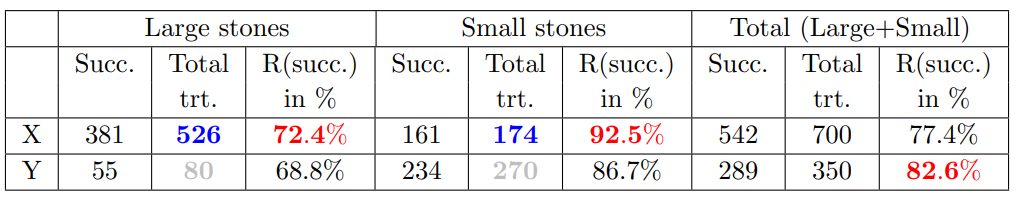
\includegraphics[width=0.75\linewidth]{images/cahpter2-simpson-rule-slicing-example.png}
        \caption{Slicing based on stone size}
        \label{fig:simpson-rule-example}
    \end{figure}
    Here, we can observe that in both large size and small size group, the rate(Success | X) > rate(Success | Y). However, after we combine these two subgroups, rate(Success | X) < rate(Success | Y). Thus, a Simpson's Paradox has appeared! But why?
    \begin{enumerate}
        \item Let us look at the numbers highlighted in blue in the table. A crucial observation at this point is that treatment X seems to be used to treat mostly patients with large stones as compared to small stones. Thus, by the \textbf{basic rule on rates}, we know that the overall success rate of treatment X will be \textbf{closer} to the large stones success rate of 72.4\% than the small stones success rate of 92.5\%. Indeed, we have the overall treatment X success rate to be 77.4\%.
        \item Similarly, the overall success rate of treatment Y will be closer to the small stones success rate 86.7\%. Indeed, the overall success rate of treatment Y is 82.6\%.
        \item Combining these two observations, it is no wonder that we have the overall success rate of X to be lower than the overall success rate of Y.
    \end{enumerate}
    \textbf{Conclusion:} Slicing the data into the small and large stone subgroups reveals that treatment X is indeed a better treatment!
\end{exbox}
\subsection{A brief introduction to confounder}
Let's take a brief look from the example above. In this example, we have introduced a third variable ``large stone size'', which is used to slice the whole original population. And based on some analysis, we will find out that the variable ``large stone size'' has association with \textbf{both} of the variables whose relationship we were initially investigating, thus affecting the conclusion of our initial study. Such a variable is called a \textit{confounder}. We will discuss more about it in the later section.
\begin{notebox}
    \begin{remark}
        When a Simpson's Paradox is observed, it implies that there is \textbf{definitely} a confounding variable present. However, the existence of a confounder does not necessarily lead to us observing Simpson's Paradox.
    \end{remark}
\end{notebox}

\section{Confounders}
\begin{dfnbox}{Confounders}{dfn-confounders}
    A {\color{red} \textbf{confounder}} is a third variable that is \textbf{associated} with both the independent and dependent variables whose relationship we are investigating.
\end{dfnbox}
\begin{notebox}
    \begin{remark}
        Note that we do not specify the direction (positive or negative) of association here. As long as the variable is associated in some way to the main variables, we will call it a \textit{confounder}, or a \textit{confounding variable}.
    \end{remark}
\end{notebox}
\subsection{Application of confounders}
The application of confounders can be summarized as follows:
\begin{enumerate}
    \item \textbf{Importance of Data Collection}: Collecting data on \textbf{potential confounders} (e.g., stone size in a medical study) is critical to identify and adjust for hidden variables that distort associations between treatment and outcome. Without this data, confounding effects remain undetected, leading to biased conclusions.
    \item \textbf{Practical Challenges}:
    \begin{itemize}
        \item \textbf{Cost and Complexity}: Gathering additional variables is often resource-intensive.
        \item \textbf{Analytical Overload}: Even with sufficient data, controlling for multiple confounders complicates analysis (e.g., "slicing" data across many variables).
    \end{itemize}
    \item \textbf{Limitations in Observational Studies}: 
    \begin{itemize}
        \item Observational studies (non-randomized) inherently face uncontrolled confounding because groups being compared (e.g., treated vs. untreated) differ in ways beyond the treatment itself.
        \item Despite adjusting for known confounders, \textbf{residual confounding} (unmeasured or unknown variables) can persist.
        \item Thus, observational studies can only establish association, not causation, as causality requires eliminating all confounder influence.
    \end{itemize}
\end{enumerate}

\subsection{A solution to confounding}
To solve the issue caused by the confounding variable, we can utilize the method of \textbf{randomization} (a.k.a randomized assignment). Why?

Recall that confounders arise when variables are \textbf{unequally distributed} between groups, leading to biased associations between the treatment and the outcome. For example, in the kidney stones study, stone size became a confounder because patients with larger stones were more likely to receive treatment X than treatment Y.

So, randomization is useful in this context because it ensures that both known and unknown confounders are, on average, equally distributed across all treatment groups. This balanced allocation eliminates the systematic relationship between any potential confounder and the treatment assignment, thereby isolating the treatment effect and minimizing bias in the results.

For example, if the allocation of large (and small) stone size cases to the two treatment types was \textbf{done randomly}, which tends to result in an equal proportion across the two groups, there would no longer be any association between stone size and treatment type. In this case, stone size would no longer be a confounder.

While randomization effectively balances confounders, it can raise ethical concerns. For instance, assigning treatments by a coin toss may compromise patient autonomy by removing their choice, which is critical in healthcare decisions. When ethical issues prevent true randomization, researchers must rely on alternative methods, such as adjusting for suspected confounders.

\begin{notebox}
    \begin{remark}
        Note that a confounding variable is associated to \textbf{both} the independent and dependent variables, so removing one of the associations is enough to remove the confounding variable.
    \end{remark}
\end{notebox}

\chapter{Dealing with Numerical Data}
\section{Univariate EDA}
\begin{dfnbox}{Distribution}{dfn-distribution}
    A {\color{red} \textbf{distribution}} is an orientation of data points, broken down by their \textbf{observed number} or \textbf{frequency of occurrence}\footnote{That's why we can think distribution as a kind of frequency table}.
\end{dfnbox}
Before we go on, let's take a look at the dataset that we will be using in this chapter,
\begin{figure}[H]
    \centering
    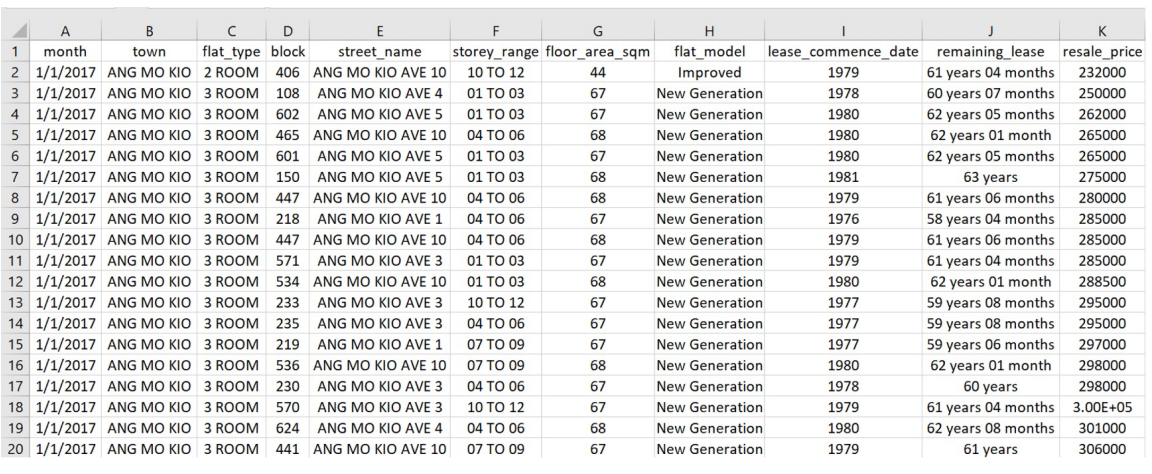
\includegraphics[width=0.75\linewidth]{images/chapter3-dataset-excel.png}
    \caption{Singapore HDB resale flats within the period of Jan 2017 to June 2021}
    \label{fig:chapter3-dataset}
\end{figure}
\begin{notebox}
    \begin{remark}
        \textbf{distribution} is often used on \textbf{one variable}.
    \end{remark}
\end{notebox}
\begin{exbox}{Distribution Example}{example-distribution}
    In this example, we want to investigate the distribution of the \textbf{Age} variable. So, we can get the following frequency table.
    \begin{figure}[H]
        \centering
        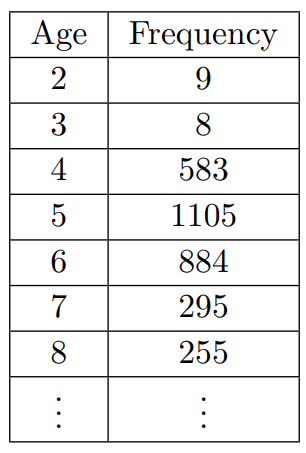
\includegraphics[width=0.15\linewidth]{images/chapter3-distribution-example.png}
        \caption{Distribution of Age}
        \label{fig:chapter3-distribution-example}
    \end{figure}
\end{exbox}
However, looking only at the frequency table, it's hard to filter out the valuable information. So, here we introduce a more ``graphical'' way -- histogram.

\subsection{Histogram}
\begin{dfnbox}{Histogram}{dfn-histogram}
    A \textbf{\color{red}{histogram}} is a \textit{graph} that groups data into \textbf{bins} (intervals) on the x-axis, with the y-axis showing the \textbf{frequency} or \textbf{count} of data points in each bin.
\end{dfnbox}
\begin{exbox}{Histogram Example}{example-histogram}
    So, to put the frequency table we have in example \ref{ex:example-distribution} into a histogram, we can use either Excel or Radiant to generate the histogram as follows,
    \begin{figure}[H]
        \centering
        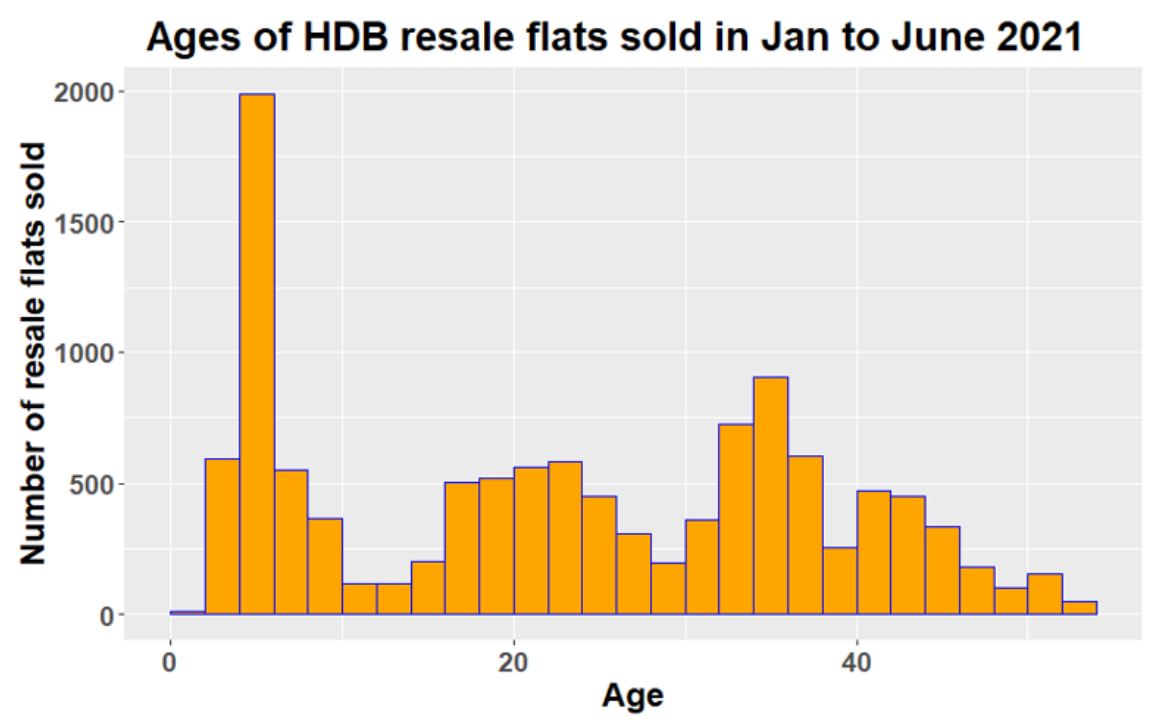
\includegraphics[width=0.6\linewidth]{images/chapter3-histogram-example.png}
        \caption{Histogram of Age}
        \label{fig:chapter3-histogram-example}
    \end{figure}
\end{exbox}
Once we have obtained a histogram, we are interested in its \textbf{overall pattern} and \textbf{deviation}
\begin{enumerate}
    \item \textbf{Overall pattern}
    \begin{enumerate}
        \item Shape
        \item Center
        \item Spread of the distribution
    \end{enumerate}
    \item \textbf{Deviation}: identify the \textit{outliers}
\end{enumerate}
\subsubsection{Shape}
There are two important descriptors when we discuss the shape of a distribution, namely the \textit{peaks} and the \textit{skewness}.
\begin{enumerate}
    \item \textbf{Peak}: Peak in a histogram highlight \textbf{the most common values} in specific intervals, which helps identify where the data is \textbf{most concentrated}. (We can think it as the local maximum in Math)
    \begin{itemize}
        \item \textbf{Unimodal Distribution}: Has a \textit{single}, distinct \textbf{peak}.
        \item \textbf{Multimodal Distribution}: Contains \textbf{multiple} peaks.
        \item \textbf{Bimodal Distribution}: A special case of multimodal distributions with exactly \textbf{two} peaks.
    \end{itemize}
    \item \textbf{Skewness}: For \textbf{unimodal distribution}, we can use another descriptor called \textit{skewness} to describe the shape of the distribution. The following is three types of skewness. \\
    \begin{figure}[H]
        \centering
        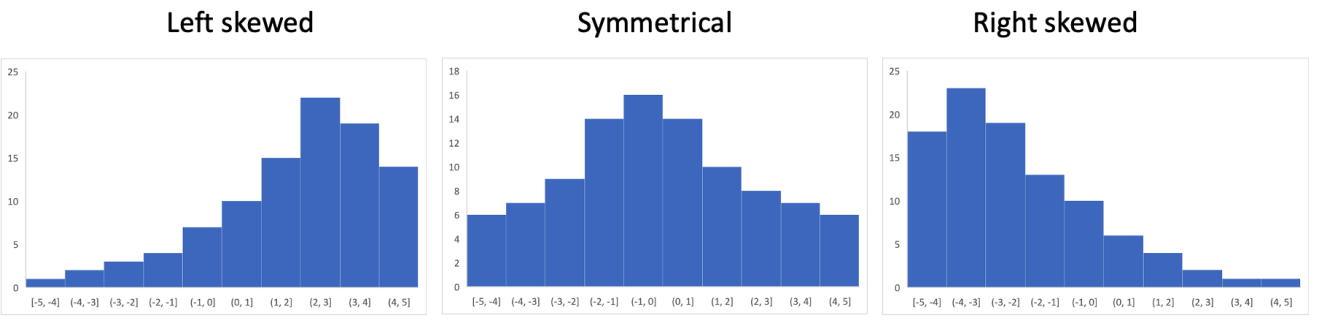
\includegraphics[width=0.65\linewidth]{images/chapter3-skewness.png}
        \caption{Skewness}
        \label{fig:chapter3-skewness}
    \end{figure}
    \begin{itemize}
        \item \textbf{Normal Distribution}: The \textit{normal distribution} is a famous \textbf{symmetrical} distribution, which is commonly known as the bell-curve.
    \end{itemize}
\end{enumerate}

\subsubsection{Central}
In this part, we are more interested in the \textbf{central tendency}, which refers to statistical measures like the mean, median, and mode that identify the central or most typical value in a data distribution. The following is the central tendency for the three skewness
\begin{figure}[H]
    \centering
    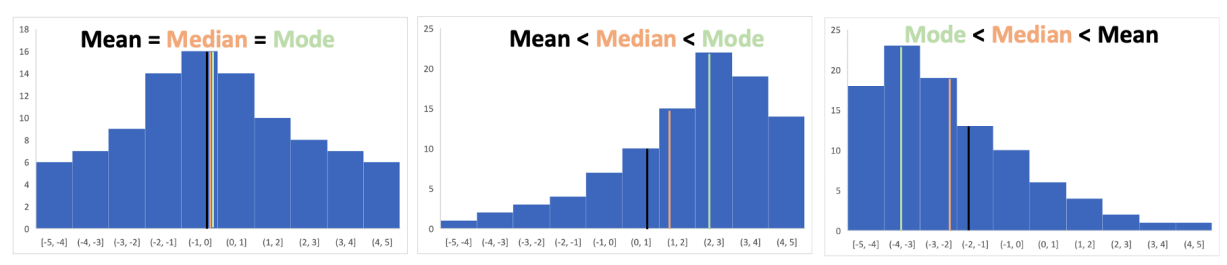
\includegraphics[width=0.9\linewidth]{images/chapter3-central-tendancy.png}
    \caption{Central Tendency}
    \label{fig:chapter3-central-tendency}
\end{figure}
\begin{notebox}
    \begin{remark}
        These three rules usually hold, but \textbf{not always} hold.
    \end{remark}
\end{notebox}

\subsubsection{Spread}
This spread of a distribution refers to how the data \textbf{vary around the central tendency}. To study the spread, we will use \textbf{standard deviation} and \textbf{range}.
\begin{enumerate}
    \item \textbf{Standard Deviation}: This has been introduced in the previous chapter.
    \item \textbf{Range}: $\text{range}=\text{the largest data point} - \text{the smallest data point}$
\end{enumerate}

\subsubsection{Outlier}
\begin{dfnbox}{Outlier}{dfn-outlier}
    An \textit{outlier} is an observation that falls well above or below the overall \textbf{bulk} of the data.
\end{dfnbox}
\begin{notebox}
    \begin{remark}
        Sometimes, we should not remove \textit{outliers} because they do convey some useful information.
    \end{remark}
\end{notebox}
In general, we should keep the following tips when deciding the \textbf{bin width} of a histogram.
\begin{enumerate}
    \item Avoid histograms with bin widths that are too large.
    \item Avoid histograms with bin widths that are too small.
    \item Our initial choice of bin width may not be the most appropriate.
\end{enumerate}
\subsubsection{Histogram vs. Bar Chart}
\textbf{Histogram}:
\begin{itemize}
    \item Depicts the distribution of a \textbf{numerical} variable along a continuous number line.
    \item Bars \textbf{touch} each other, reflecting adjacent numeric intervals.
    \item The order of bars \textbf{cannot} be changed because they represent a progression of numeric values.
\end{itemize}
\textbf{Bar Chart}:
\begin{itemize}
    \item Displays data for \textbf{categorical} variables, where each bar corresponds to a distinct category.
    \item Bars typically have \textbf{gaps} between them.
    \item The order of bars can be \textbf{rearranged} freely without affecting the interpretation of the data.
\end{itemize}

\subsection{Boxplot}
Besides histogram, we can use \textbf{boxplot} to visualize the distribution of a numerical variable. To construct a boxplot, we need to following five numbers,
\begin{enumerate}
    \item Minimum
    \item Quartile 1(Q1)
    \item Median (Q2)
    \item Quartile 3(Q3)
    \item Maximum
\end{enumerate}
Furthermore, we also need to calculate the Interquartile range (IQR). While median can be viewed as the center of a data set, the IQR is a way to quantify the \textbf{spread} of a data set.
\begin{displaymath}
    \text{IQR}=Q_3-Q_1
\end{displaymath}
After that, we can use a mathematical way to decide which points are \textit{outliers}. This is done using the following theorem
\begin{thmbox}{Find Outliers}{thm-find-outliers}
    A data point is considered an {\color{red} \textbf{outlier}} if it satisfies \textbf{one} of the following conditions:
    \begin{itemize}
        \item The value of the data point is \textbf{greater than} $Q_3+1.5\times\text{IQR}$
        \item The value of the data point is \textbf{less than} $Q_1-1.5\times\text{IQR}$
    \end{itemize}
\end{thmbox}
To construct the boxplot, we can follow the 5 steps below
\begin{enumerate}
    \item Draw a box from $Q_1$ to $Q_3$
    \item Draw a vertical line in the box where the median ($Q_2$) is located
    \item Identify all the outliers by using the theorem \ref{thm:thm-find-outliers} above.
    \item Extend a line from $Q_1$ to the \underline{smallest value that is \textbf{not} an outlier} and another line from $Q_3$ to the \underline{largest value that is \textbf{not} an outlier}. These lines are called \textit{whiskers}
    \item Mark each of the outliers with dots or asterisks.
\end{enumerate}
\begin{figure}[H]
    \centering
    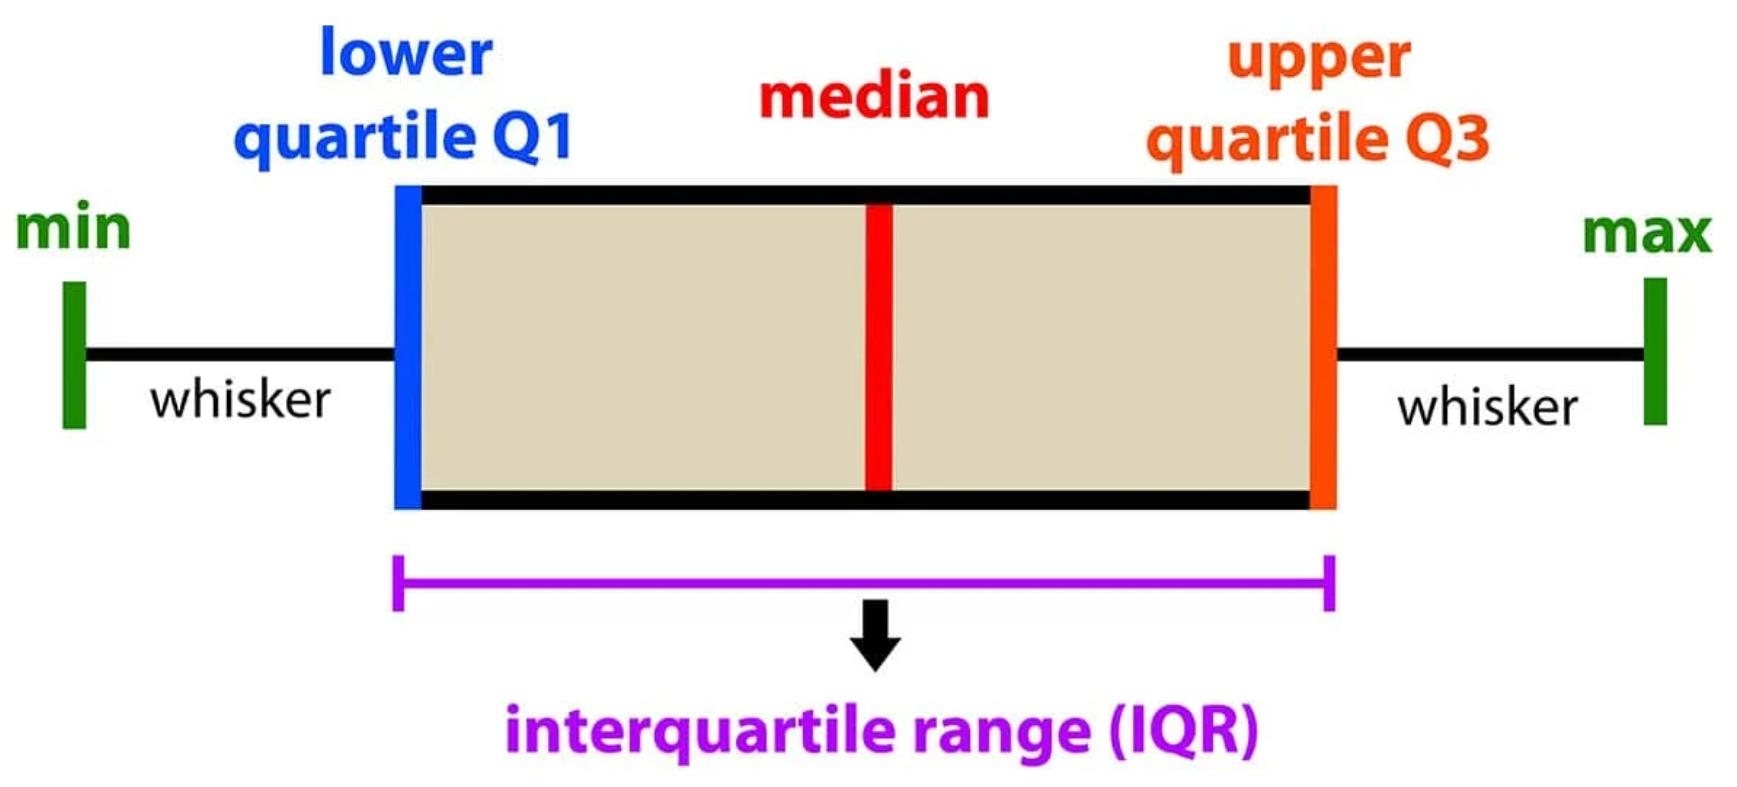
\includegraphics[width=0.75\linewidth]{images/chapter3-boxplot-example.png}
    \caption{Boxplot Explanation}
    \label{fig:chapter3-boxplot-explanation}
\end{figure}
\subsubsection{Boxplot vs. Histogram}
\begin{enumerate}
    \item A \textbf{histogram} typically gives a better sense of the \textit{shape} of the \textbf{distribution} of a variable, compared to a \textbf{boxplot}.
    \item If we wish to compare the \textbf{distributions} of different \textbf{data sets}, putting the different \textbf{boxplots} side by side is more illustrative than using \textbf{histograms}.
    \item To identify and indicate \textbf{outliers}, \textbf{boxplots} do a better job than \textbf{histograms}.
    \item The number of \textbf{data points} we have in a \textbf{data set} is better shown in a \textbf{histogram} than in a \textbf{boxplot}.
\end{enumerate}

\section{Bivariate EDA}
In this section, we will be focusing on studying the \textbf{Bivariate\footnote{Bivariate data is data involving two variables.} EDA}, especially the \textbf{relationship between two variables}. And based on the relationship, we can divide this section into two parts,
\begin{enumerate}
    \item Deterministic relationship
    \item Non-deterministic or statistical relationship
\end{enumerate}
\subsection{Deterministic}
\begin{dfnbox}{Deterministic}{dfn-deterministic}
    {\color{red} \textbf{Deterministic}} means that the value of one variable can be \textbf{determined exactly} (this means that the determined value is unique) if we know the value of the other variable.
\end{dfnbox}
The most common type of deterministic relationship is the one that involves the conversion of units of measurement from one metric to another.
\begin{exbox}{Deterministic Relationship Example}{example-deterministic-relationship}
    For example, the relationship between Fahrenheit (F) and Degree Celsius (C) in the measurement of temperature is \textbf{deterministic}. \\
    \textbf{Solution}: The relationship can be written as:
    \begin{equation*}
        C=(F-32)\times \frac{5}{9}
    \end{equation*}
\end{exbox}

\subsection{Non-deterministic}
However, as we have said before, the main focus of this section is on a relationship between two variables that is not deterministic in nature. This is also more common in our daily life.
\begin{dfnbox}{Non-deterministic}{dfn-non-deterministic}
    {\color{red} \textbf{Non-deterministic\footnote{``Non-deterministic'' is sometimes referred to as ``statistical''}}} means that when given the value of one variable, we can only describe the \textbf{average value} of the other variable. And this kind of relationship is also called \textbf{association}.
\end{dfnbox}
When doing the Bivariate EDA, we may find that unlike Univariate data, a frequency table, a boxplot or a hitogram is less useful for showing associations between two variables. So, in Bivariate EDA, we will mainly do,
\begin{enumerate}
    \item \textbf{Scatter Plot}: For better visualization in Bivariate Data, a scatter plot is used to visualize the relationship between the two variables by displaying \textbf{data points}.
    \item \textbf{Correlation Coefficient}: After examining the scatter plot, a correlation coefficient quantifies the \textbf{strength and direction} of any \textbf{linear association}.
    \item \textbf{Regression Analysis}: Finally, regression analysis fits a line or curve through the data points, allowing for predictions of one variable based on the other.
\end{enumerate}
\begin{notebox}
    \begin{remark}
        Note the \textbf{regression} is used to predict, we \textbf{cannot} use the correlation coefficient to predict!
    \end{remark}
\end{notebox}

\subsection{Scatter Plot}
\begin{dfnbox}{Scatter Plot}{dfn-scatter-plot} 
    A \textbf{scatter plot} is a graphical tool that displays pairs of data values for two variables as individual points on a coordinate system. The overall pattern of these points helps reveal the type and strength of the \textbf{association} between the variables.
\end{dfnbox}
\begin{notebox}
    \begin{remark}
        In Scatter plot, the x-axis is your \textbf{independent variable}, the y-axis is your \textbf{dependent variable}.
    \end{remark}
\end{notebox}
For example, we will be studying the \textbf{age} and \textbf{resale price} in Figure \ref{fig:chapter3-dataset}, and the following will be an example of what our scatter plot looks like,
\begin{figure}[H]
    \centering
    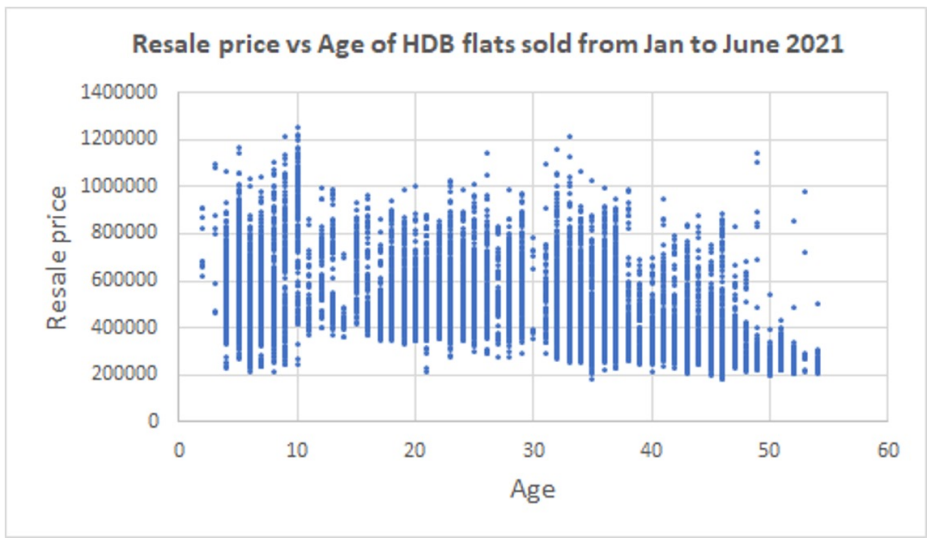
\includegraphics[width=0.6\linewidth]{images/chapter3-scatter-plot-example.png}
    \caption{Scatter Plot Example}
    \label{fig:chapter3-scatter-plot-example}
\end{figure}
So, now how should we look at our scatter plot? Below is the table that summarizes the difference between what we should look from Univariate data and Bivariate data.
\begin{table}[h]
\centering
\begin{tabular}{|p{3cm}|p{3cm}|p{3cm}|p{3cm}|}
\hline
\multicolumn{2}{|c|}{\textbf{Univariate data}} & \multicolumn{2}{c|}{\textbf{Bivariate data}} \\
\hline
\textbf{Overall pattern} & \textbf{Deviation} & \textbf{Overall pattern} & \textbf{Deviation} \\
\hline
\begin{tabular}[c]{@{}l@{}}
1) Shape\\
2) Center\\
3) Spread
\end{tabular}
& Outliers
& \begin{tabular}[c]{@{}l@{}}
1) Direction\\
2) Form\\
3) Strength
\end{tabular}
& Outliers \\
\hline
\end{tabular}
\caption{Comparison of univariate and bivariate data characteristics}
\label{tab:chapter3-univariate-bivariate}
\end{table} \\
From the table above, we can clearly see that
\begin{enumerate}
    \item \textbf{Univariate Data}: the key descriptors are \textbf{Shape} (symmetrical/skewed), \textbf{Center} (median, mean, mode), \textbf{Spread} (interquartile range, standard deviation, range).
    \item \textbf{Bivariate Data}: the key descriptors are \textbf{Direction}, \textbf{Form}, \textbf{Strength} of the association.
    \item \textbf{Common Aspect}: Data points that significantly deviate from the main pattern are \textbf{outliers}.
\end{enumerate}
\subsubsection{Direction}
\begin{dfnbox}{Direction}{dfn-direction}
    {\color{red} \textbf{Direction}} describes the nature of the relationship between two variables: a \textbf{positive} relationship means that increases in one variable correspond to \textbf{increases} in the other; a \textbf{negative} relationship means that increases in one variable correspond to \textbf{decreases} in the other; if neither pattern is observed, the relationship has no specific direction.
\end{dfnbox}
For example, below is an example of the \textbf{direction} in the scatter plot.
\begin{figure}[H]
    \centering
    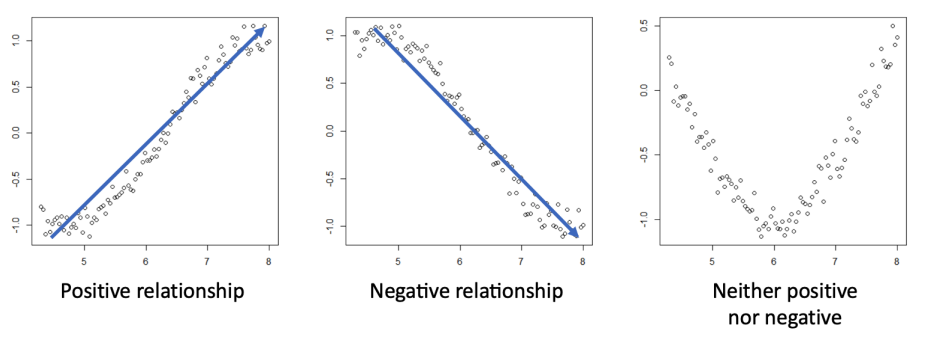
\includegraphics[width=0.75\linewidth]{images/chapter3-scatter-plot-direction.png}
    \caption{Scatter Plot Direction}
    \label{fig:chapter3-scatter-plot-direction}
\end{figure}
\begin{notebox}
    \begin{remark}
        Not all relationships can be classified as either positive or negative and there are those that do not behave in one way or the other.
    \end{remark}
\end{notebox}
\subsubsection{Form}
\begin{dfnbox}{Form}{dfn-form}
    The {\color{red} \textbf{form}} of the relationship describes the overall shape of a scatter plot. It is classified as \textbf{linear} when the data points cluster around a straight line, and as \textbf{non-linear} when they form a smooth curve (e.g., quadratic or exponential patterns).
\end{dfnbox}
For example, below is an example of the \textbf{form} in the scatter plot.
\begin{figure}[H]
    \centering
    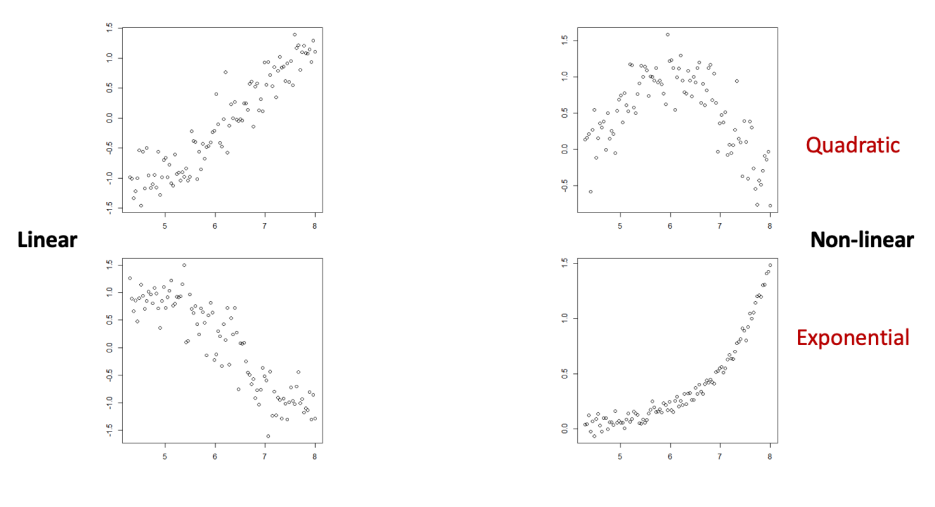
\includegraphics[width=0.75\linewidth]{images/chapter3-scatter-plot-form.png}
    \caption{Scatter Plot Form}
    \label{fig:chapter3-scatter-plot-form}
\end{figure}
The two scatter plots on the left shows a linear form of the relationship between the two variables while the two scatter plots on the right shows non-linear forms
\subsubsection{Strength}
\begin{dfnbox}{Strength}{dfn-strength}
    The {\color{red} \textbf{strength}} of the relationship indicates \textbf{how closely} the data follow the \textbf{form} of the relationship.
\end{dfnbox}
For example, below is an example of the \textbf{strength} in the scatter plot.
\begin{figure}[H]
    \centering
    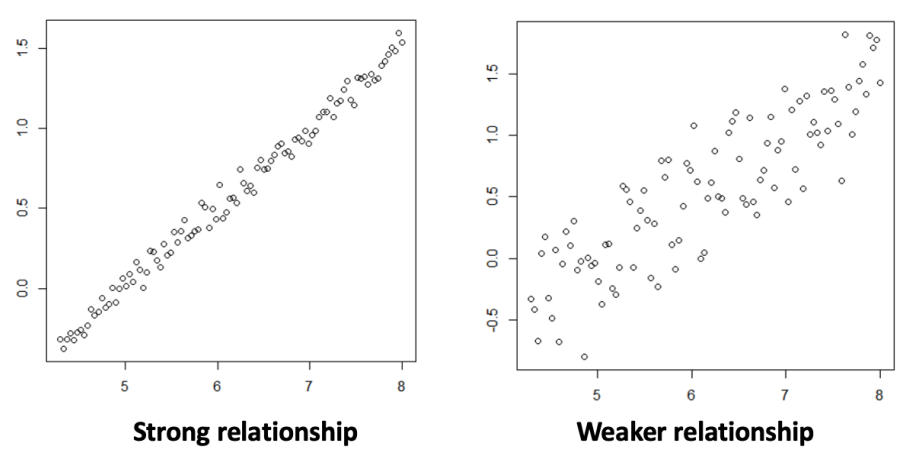
\includegraphics[width=0.7\linewidth]{images/chapter3-scatter-plot-strength.png}
    \caption{Scatter Plot Strength}
    \label{fig:chapter3-scatter-plot-strength}
\end{figure}

\subsection{Correlation Coefficient}
\begin{dfnbox}{Correlation}{dfn-correlation}
    The {\color{red} \textbf{correlation coefficient}} between two numerical variables is a measure of the \textbf{linear} association between them. The correlation coefficient, denoted by $r$, always ranges between -1 and 1. 
\end{dfnbox}
We can use $r$ to summarize the \textbf{direction and strength} of linear association between two variables.
\begin{enumerate}
    \item If \(r > 0\), the association is \textbf{positive}: an increase in one variable is associated with an increase in the other.
    \item If \(r < 0\), the association is \textbf{negative}: an increase in one variable is associated with a decrease in the other.
    \item \(r = 1\) indicates \textbf{perfect positive association}; \(r = -1\) indicates \textbf{perfect negative association}.
    \item \(r = 0\) signifies \textbf{no linear association}.
    \item The \textbf{sign} of \(r\) reveals the direction, while the \textbf{magnitude} (how close \(r\) is to 1 or \(-1\)) indicates the \textbf{strength} of the association.
\end{enumerate}
\begin{notebox}
    \begin{remark}
        \textbf{No linear association} between variables does not necessarily mean no association between variables. The relationship can be \textbf{non-linear} also, like the form of \textbf{quadratic} we have seen previously.
    \end{remark}
\end{notebox}
When describing the \textbf{strength} of a linear relationship, we usually follow the rule of thumb as given in the diagram below,
\begin{figure}[H]
    \centering
    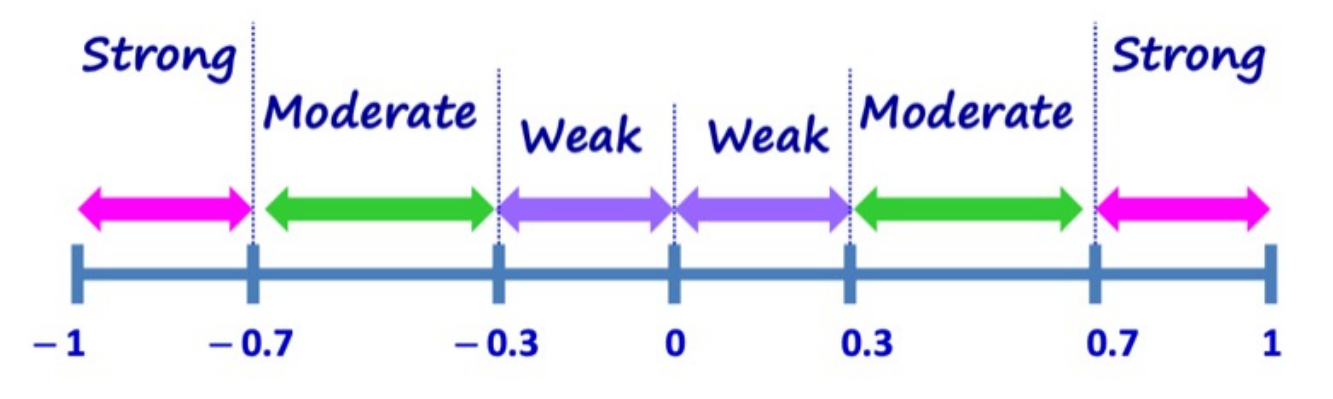
\includegraphics[width=0.75\linewidth]{images/chapter3-correlation-coefficient-rule-of-thumb.png}
    \caption{Correlation Coefficient Rule of Thumb}
    \label{fig:chapter3-correlation-coefficient-rule-of-thumb}
\end{figure}
\subsubsection{Compute the correlation coefficient $r$}
The first method is to compute $r$ \textbf{by hand} (\textbf{not recommended})

To do so, let's use the table that shows a total of 10 data points of Bivariate data $(x,y)$
\begin{table}[h]
\centering
\begin{tabular}{|c|c|c|c|c|c|c|c|c|c|c|}
\hline
\textbf{x} & 9 & 4 & 5 & 10 & 6 & 3 & 7 & 2 & 8 & 1 \\
\hline
\textbf{y} & 41 & 17 & 28 & 50 & 39 & 26 & 30 & 6 & 4 & 10 \\
\hline
\end{tabular}
\caption{Sample (x, y) data}
\label{tab:chapter3-xy-data}
\end{table}
\begin{enumerate}
    \item \textbf{First compute the mean and standard deviation of $x$ and $y$}: For this dataset, we find the mean and standard deviation of $x$ to be 5.5 and 3.03 respectively while the mean and standard deviation of $y$ are 25.1 and 15.65 respectively.
    \item \textbf{Convert each value of $x$ and $y$ into \textit{standard units}}: To convert $x$ (resp. $y$) into its standard unit, we compute
    \begin{equation}
        \frac{x-\bar{x}}{s_x}~~(\text{resp.}\frac{y-\bar{y}}{s_y})
    \end{equation}
    where $s_x$ and $s_y$ are the standard deviations of $x$ and $y$ respectively. The table \ref{tab:chapter3-standardized_values} below shows the values of $x$ and $y$ after they have been converted to standard units.
    \begin{table}[h]
        \centering
        \renewcommand{\arraystretch}{1.2} % Adjust row height for better readability
        \begin{tabular}{|c|c|c|c|c|c|c|c|c|c|c|}
        \hline
        $x$ & 1.16 & -0.50 & -0.17 & 1.49 & 0.17 & -0.83 & 0.50 & -1.16 & 0.83 & -1.49 \\
        \hline
        $y$ & 1.02 & -0.52 & 0.19 & 1.59 & 0.89 & 0.06 & 0.31 & -1.22 & -1.35 & -0.96 \\
        \hline
        \end{tabular}
        \caption{Standardized (x, y) values}
        \label{tab:chapter3-standardized_values}
    \end{table}
    \item \textbf{Compute the product $xy$ in their standard units for each data point}: The table \ref{tab:chapter3-xy_values} below has an additional row for the value $xy$ for each data point.
    \begin{table}[h]
        \centering
        \renewcommand{\arraystretch}{1.2} % Adjust row height for better readability
        \begin{tabular}{|c|c|c|c|c|c|c|c|c|c|c|}
        \hline
        $x$  & 1.16  & -0.50  & -0.17  & 1.49  & 0.17  & -0.83  & 0.50  & -1.16  & 0.83  & -1.49  \\
        \hline
        $y$  & 1.02  & -0.52  & 0.19  & 1.59  & 0.89  & 0.06  & 0.31  & -1.22  & -1.35  & -0.96  \\
        \hline
        $xy$ & 1.17  & 0.26   & -0.03  & 2.36  & 0.15  & -0.05  & 0.15  & 1.41   & -1.11  & 1.43   \\
        \hline
        \end{tabular}
        \caption{Values of $x$, $y$, and their product $xy$}
        \label{tab:chapter3-xy_values}
    \end{table}
    \item \textbf{Sum the products $xy$ obtained in the previous step over all the data points and then divide the sum by $n-1$, where $n$ is the number of data points. The result is the correlation coefficient $r$}: For the data set above,
    \begin{equation*}
        r=\frac{1}{9}(1.17+0.26-0.03+2.36+0.15-0.05+0.15+1.41-1.11+1.43)=0.64
    \end{equation*}
\end{enumerate}
\begin{notebox}
    \begin{remark}
        For the purpose of this course, you are not required to calculate the correlation coefficient by hand. However, by knowing this calculation method, you may develop some basic intuition on the properties of $r$
    \end{remark}
\end{notebox}
The second method is to use the calculator to get the correlation coefficient $r$. \\
(\textbf{Recommended})
\subsubsection{Properties of correlation coefficient $r$}
\begin{thmbox}{Properties of Correlation Coefficient $r$}{thm-property-r}
    \begin{enumerate}
        \item $r$ is \textbf{not} affected by \textbf{interchanging} the $x$ and $y$ variables.
        \item $r$ is \textbf{not} affected by \textbf{adding} a number to \textbf{all} values of a variable.
        \item $r$ is \textbf{not} affected by \textbf{multiplying} a \textbf{positive} number to \textbf{all} values of a variable.
    \end{enumerate}
\end{thmbox}
\textbf{Explanation}:
\begin{enumerate}
    \item \textbf{Interchanging \( x \) and \( y \) does not affect \( r \)}  
    \begin{itemize}
        \item The formula for \( r \) is:
        \[
        r = \frac{1}{n-1} \sum \left( \frac{x - \bar{x}}{s_x} \times \frac{y - \bar{y}}{s_y} \right)
        \]
        \item Since multiplication is commutative, swapping \( x \) and \( y \) does not change the sum, meaning \( r \) remains the same.
    \end{itemize}
    
    \item \textbf{Adding a constant to all values of \( x \) or \( y \) does not affect \( r \)}  
    \begin{itemize}
        \item Adding a constant \( c \) shifts the mean by \( c \), but does not change the standard deviation \( s_x \) or \( s_y \), since it only affects location, not spread.
        \item The standardized values \( (x - \bar{x})/s_x \) remain unchanged, so \( r \) remains the same.
    \end{itemize}

    \item \textbf{Multiplying all values by a positive constant does not affect \( r \)}  
    \begin{itemize}
        \item Scaling \( x \) or \( y \) by a positive factor \( k \) scales both the numerator and denominator in standardization:
        \[
        \frac{kx - k\bar{x}}{ks_x} = \frac{x - \bar{x}}{s_x}
        \]
        \item Since standard units remain unchanged, the correlation coefficient \( r \) remains unaffected.
    \end{itemize}
\end{enumerate}
\begin{notebox}
    \textit{Remark.}
    \begin{enumerate}
        \item \textbf{Association is not causation}: With $r$ being close to 1 or -1, we can only say there is a \textbf{strong association} between these two variables, and this is a \textit{statistical relationship} between $x$ and $y$ instead of a \textit{causal relationship}.
        \item \textbf{$r$ does not tell us anything about non-linear relationship}: $r$ only measures the degree of \textbf{linear association} between two variables. For example,
        \begin{figure}[H]
            \centering
            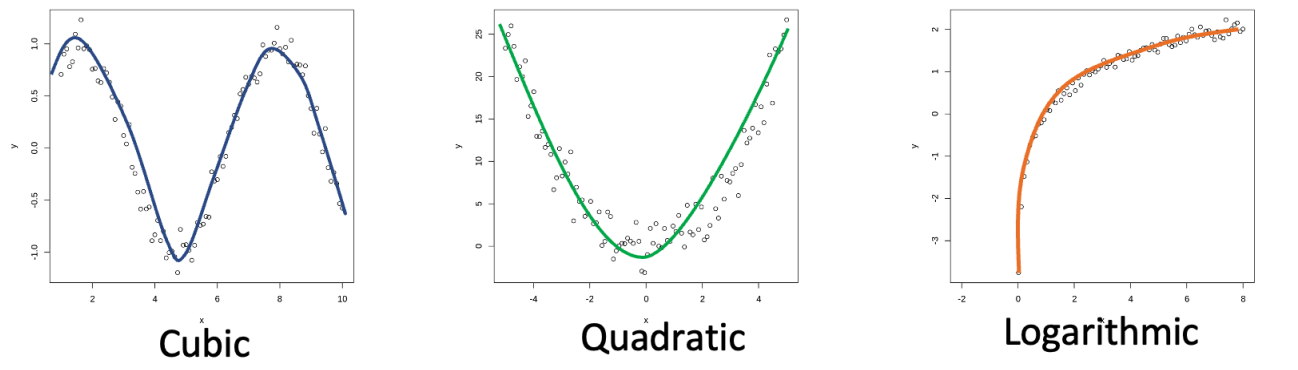
\includegraphics[width=0.75\linewidth]{images/chapter3-r-and-non-linear-association.png}
            \caption{Non-linear association}
            \label{fig:chapter3-r-and-non-linear-association}
        \end{figure}
        The correlation coefficient $r$ for these three scatter plots above are small but yet there is actually a \textbf{strong} relationship between variables. The value of $r$ is small because the relationship between the variables is \textbf{not a linear one}.
        \begin{notebox}
            \begin{remark}
                It is always a good practice to look at a scatter plot of the data set and not just deduce any relationship between the variables from the computed value of $r$.
            \end{remark}
        \end{notebox}
        \item \textbf{Outliers can affect the correlation coefficient significantly}
    \end{enumerate}
\end{notebox}

\subsubsection{Ecological Correlation}
\begin{dfnbox}{Ecological Correlation}{dfn-ecological-correlation}
    The {\color{red} \textbf{ecological correlation}} represents relationships observed at the \textbf{aggregate level}, considering the characteristics of \textbf{groups} rather than \textbf{individuals}.
\end{dfnbox}
Think of it this way: when we compute correlation for \textbf{individuals}, each data point captures \textbf{personal variability}. But when we group individuals into \textbf{aggregates} (e.g., city averages instead of personal incomes), we \textbf{smooth out individual differences}. This reduction in variability makes patterns seem \textbf{stronger} than they actually are. The correlation appears inflated because it reflects group trends rather than true individual relationships.
\begin{dfnbox}{Ecological Fallacy}{dfn-ecological-fallacy}
    The {\color{red} \textbf{ecological}} fallacy occurs when incorrect inferences about individual-level behavior are made based on aggregate-level data.
\end{dfnbox}
For example, the following graph shows an \textbf{ecological fallacy}. In this figure, although the aggregate subgroup averages (denoted by four red points) show a \textbf{positive} correlation, the individual-level data within each subgroup actually reveals a weak \textbf{negative} correlation. Thus, assuming a positive individual correlation based on the aggregate data would be incorrect.
\begin{figure}[H]
    \centering
    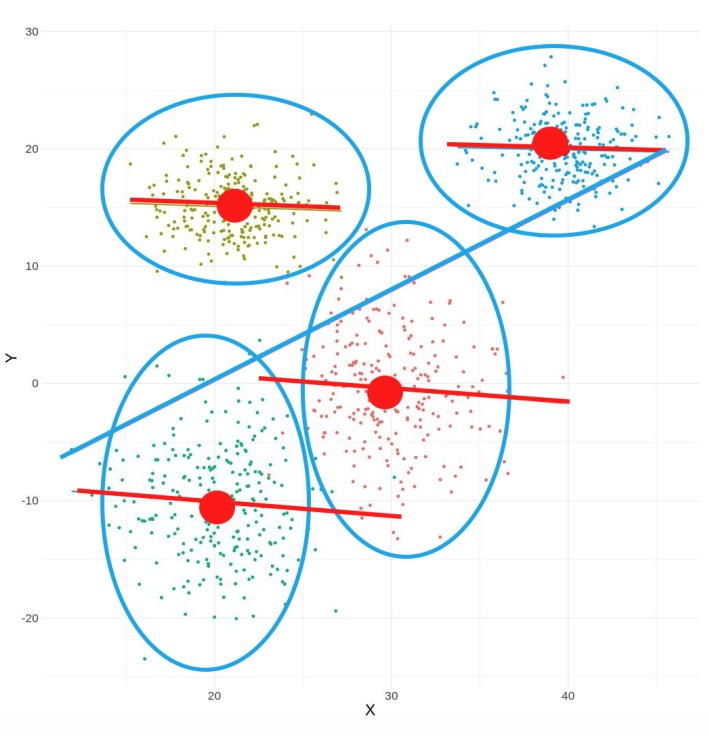
\includegraphics[width=0.3\linewidth]{images/chapter3-ecological-fallacy.png}
    \caption{Ecological Fallacy}
    \label{fig:chapter3-ecological-fallacy}
\end{figure}
\begin{dfnbox}{Atomistic Fallacy}{dfn-atomistic-fallacy}
    The {\color{red} \textbf{atomistic fallacy}} occurs when incorrect inferences about aggregate-level behavior are made based on individual-level data.
\end{dfnbox}
For example, the following graph shows an \textbf{atomistic fallacy}. From the individual-level data within each subgroup, we can see a clear positive relationship. But if we look at the aggregate subgroup averages (denoted by three red points), there is actually no relationship! Thus, an atomistic fallacy occurs!
\begin{figure}[H]
    \centering
    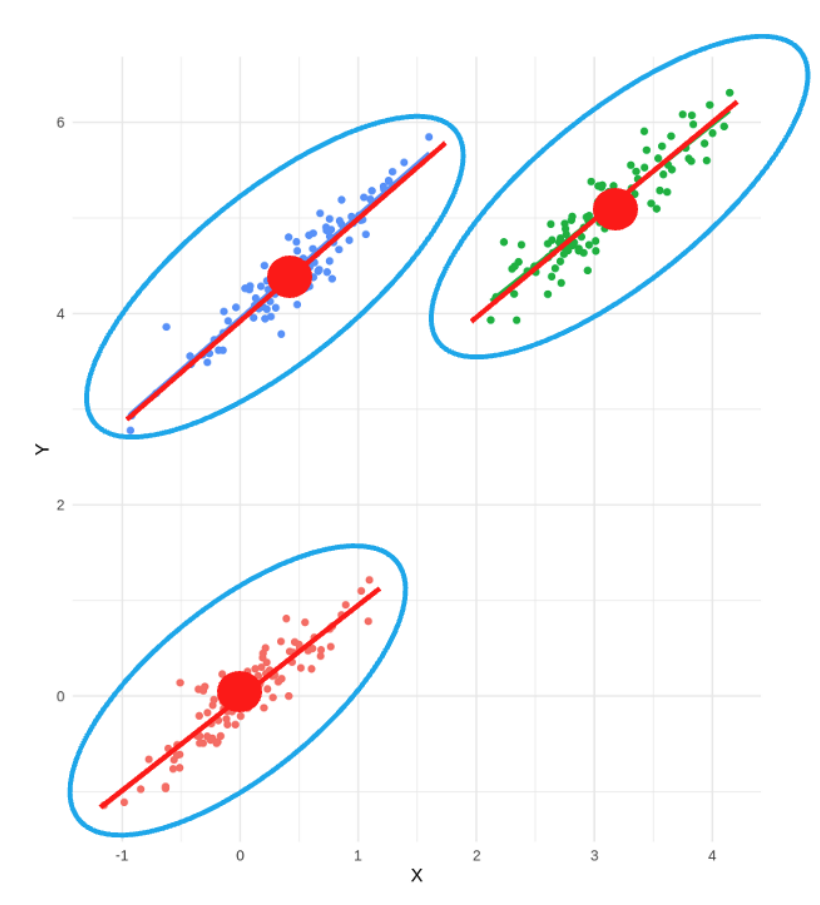
\includegraphics[width=0.3\linewidth]{images/chapter3-atomistic-fallacy.png}
    \caption{Atomistic Fallacy}
    \label{fig:chapter3-atomistic-fallacy}
\end{figure}
To sum up, the following table summarizes the difference between ecological fallacy and atomistic fallacy. \\
\begin{table}[h]
\centering
\begin{tabular}{|c|p{4.5cm}|p{4.5cm}|}
\hline
\textbf{Fallacy} & \textbf{Using} & \textbf{To Conclude} \\ \hline
Ecological & Ecological correlation (aggregate level) & Individual level correlation \\ \hline
Atomistic & Individual level correlation & Ecological correlation (aggregate level) \\ \hline
\end{tabular}
\caption{Ecological and Atomistic Fallacies}
\end{table}
\begin{notebox}
    \begin{remark}
        The aggregate level is the \textbf{subgroup average}, which is one point that represents its subgroup. The individual-level represents the \textbf{individual point within each subgroup}, \textbf{not} individual point within the \textbf{whole group}!
    \end{remark}
\end{notebox}

\subsection{Linear Regression}
\begin{dfnbox}{Linear Regression}{dfn-linear-regression}
    In this course, {\color{red} Linear regression} is a statistical method used to model the relationship between the dependent variable and the independent variable by fitting a \textbf{linear equation} ($Y=mX+b$) to observed data.
\end{dfnbox}
\begin{figure}[H]
    \centering
    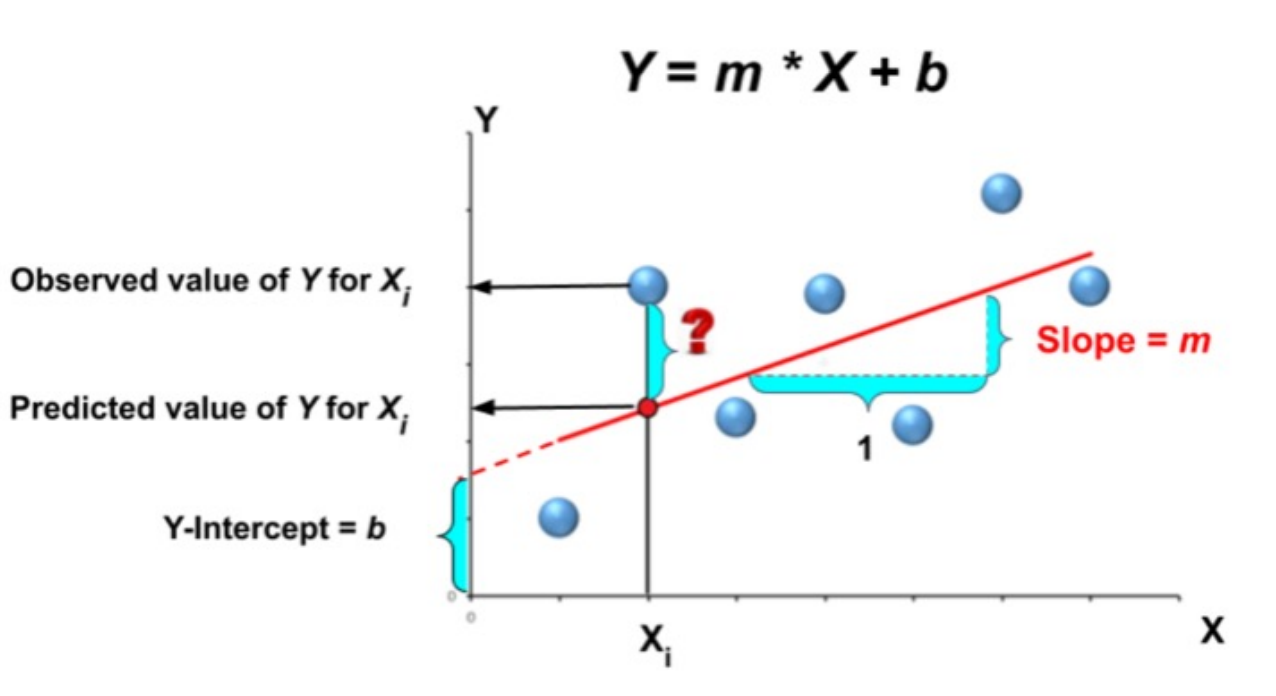
\includegraphics[width=0.5\linewidth]{images/chapter3-linear-regression.png}
    \caption{Linear Regression}
    \label{fig:chapter3-linear-regression}
\end{figure}
\begin{dfnbox}{Residual}{dfn-residual}
    From the figure \ref{fig:chapter3-linear-regression}, we define the {\color{red} \textbf{residual\footnote{This residual, denoted by $e_i$, is sometimes called the \textbf{error} of the $i$-th observation as it measures how far the predicted value is from the observed value.}}} of the $i$-th observation as the observed value of $Y$ for $X_i$ (that is, $Y_i$) minus the predicted value of $Y$ of $X_i$ (predicted by the straight line).
\end{dfnbox}
\subsubsection{The Least Squares Method}
The least squares method is a technique for finding the \textbf{best-fitting} line to a set of data points.
\begin{enumerate}
    \item \textbf{Motivation:}
    \begin{itemize}
        \item The goal is to minimize the discrepancy between the observed and predicted values.
        \item We want to find the line that best approximates the data points by reducing the error.
    \end{itemize}
    \item \textbf{Formal Definition:}
    \begin{itemize}
        \item Let the data points be \((x_1, y_1), (x_2, y_2), \dots, (x_n, y_n)\).
        \item The model is \(y = ax + b\), where \(a\) is the slope and \(b\) is the intercept.
        \item The error for each data point is \(e_i = y_i - (ax_i + b)\).
        \item The least squares objective function is the sum of squared errors:
        \[
        S(a, b) = \sum_{i=1}^{n} e_i^2 = \sum_{i=1}^{n} \left( y_i - (ax_i + b) \right)^2
        \]
    \end{itemize}
    \item \textbf{Calculation:}
    \begin{itemize}
        \item To find the optimal values of \(a\) and \(b\), take the partial derivatives of \(S(a, b)\) with respect to \(a\) and \(b\).
        \item Set the partial derivatives equal to zero and solve the resulting system of equations.
        \begin{notebox}
            \begin{remark}
                This step is usually down by the calculator or computer.
            \end{remark}
        \end{notebox}
    \end{itemize}
    \item \textbf{Why Square the Errors?}
    \begin{itemize}
        \item Squaring the errors ensures all errors contribute \textbf{positively} to the total sum.
        \item Without squaring, large positive and negative errors could cancel each other out, making the total error misleading.
        \item Squaring penalizes large deviations more heavily, resulting in a better and more robust fit.
    \end{itemize}
\end{enumerate}
\begin{notebox}
    \textit{Remark.}
    \begin{enumerate}
        \item \textbf{Always pass through the average point}: The least squares regression line obtained from a set of observed data points $(x_i, y_i)$ will \textbf{always} pass through that point of averages for that dataset, that is $(\bar{x}, \bar{y})$
        \item \textbf{Not interchangeable}: We cannot change the dependent variable and independent variable.
        \item \textbf{Difference between correlation coefficient $r$}:
        \begin{itemize}
            \item The linear regression line is a \textbf{line} while the correlation coefficient $r$ is just a \textbf{number}. (a.k.a to predict a value based on another value, we need \textbf{linear regression} instead of correlation coefficient.)
            \item The gradient of the regression line $m$ is \textbf{different from} the correlation coefficient $r$. But they share the \textbf{same sign} because of ths following relationship between them
            \begin{equation*}
                m=\frac{s_Y}{s_X}r
            \end{equation*}
            where $s_X$ (resp. $s_Y$) is the standard deviation of $X$ (resp. $Y$).
        \end{itemize}
        \item \textbf{Make prediction only within the range of dependent variable}
    \end{enumerate}
\end{notebox}
\subsubsection{Non-Linear Relationship}
Some non-linear relationship can be converted to become \textbf{linear}. For example, an exponential relationship
\begin{equation*}
    y=cb^t
\end{equation*}where $c$ and $b$ are some constants that we will determine. It can be converted to a linear relationship by taking the $\ln$ operation on both sides
\begin{equation*}
    \ln y=\ln(cb^t)\equiv\ln y=\ln c +t\ln b
\end{equation*}
Thus, if there is an exponential relationship between $y$ and $t$, then we would expect to see a \textbf{linear relationship} between $\ln y$ and $t$. And the following are the steps to determine $c$ and $b$
\begin{enumerate}
    \item For each data point $(t,y)$, compute $(t, \ln y)$
    \item Find the linear regression line for $\ln y$ vs. $t$
    \item Use the gradient and y-intercept to find the value of $c$ and $b$
    \item Rewrite the final exponential relationship
\end{enumerate}

\chapter{Statistical Inference}
\section{Statistical Inference}
\begin{dfnbox}{Statistical Inference}{dfn-statistical-inference}
    {\color{red} \textbf{Statistical inference}} refers to the use of \textbf{samples} to draw inferences or conclusions about the \textbf{population} in question.
\end{dfnbox}
Our final goal in data analysis is to generate some information about the \textbf{population}. However, from the previous chapter, we only do EDA on the \textbf{sample}. So, we are more interested in \textbf{whether similar conclusions made at the sample level can be made at the population level also}. The following graph shows how statistical inference fits into exploratory data analysis (EDA) framework.
\begin{figure}[H]
    \centering
    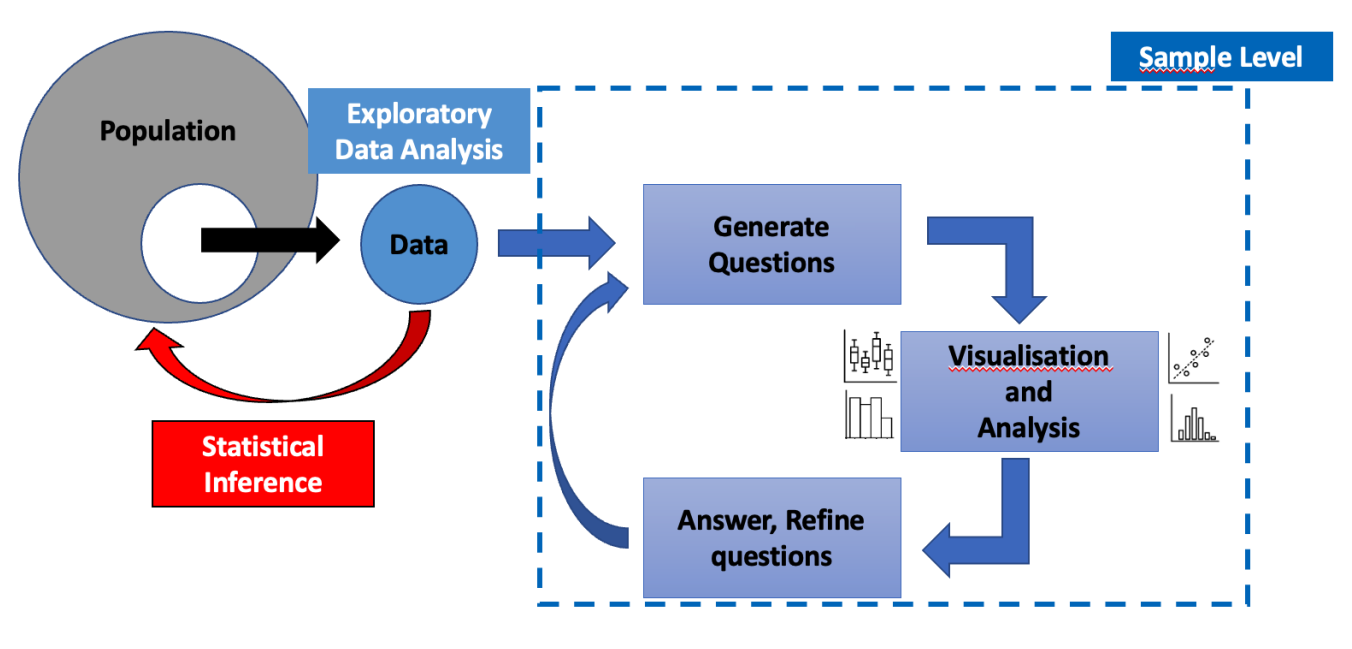
\includegraphics[width=0.6\linewidth]{images/chapter4-why-statistical-inference.png}
    \caption{Statistical inference and EDA}
    \label{fig:chapter4-why-statistical-inference}
\end{figure}
Recall that the \hyperref[dfn:dfn-population-parameter]{population parameter} is a numerical fact about the \textbf{population}. When we take a sample from the population, the use of a sample statistic to estimate the population parameter is subjected to inaccuracies, which typically include \textit{bias} and \textit{random error}.
\begin{equation*}
    \text{Sample statistic}=\text{population parameter}+\text{bias}+\text{random error}
\end{equation*}
First thing first, in order to use our sample to make inference about the population, the \textbf{fundamental rule for using data for inference} should be met.
\begin{thmbox}{Fundamental Rule for using Data for Inference}{thm-fundamental-rule-to-use-data-for-inference}
    Available data can be used to make inferences about a much larger group if the data can be considered to be \textbf{representative} with regards to the question of interest.
\end{thmbox}
By adopting good sampling method (e.g. using simple random sampling) and practices (e.g. having a good sampling frame), selection bias can be reduced. In addition, having a high response rate will minimise non-response bias. If bias can be reduced to an \textbf{insignificant level}, this would allow us to say
\begin{equation*}
    \text{Sample statistic}=\text{population parameter}+\text{random error}
\end{equation*}
The quantity of \textbf{random errors} refers to small differences that arise as a result of the sampling variability when using any probability-based sampling method.
\begin{notebox}
    \begin{remark}
        In the following content, we assume that \textbf{bias} can be reduced, so we only care about the random errors.
    \end{remark}
\end{notebox}
In this course, the statistical inference includes two types
\begin{enumerate}
    \item confidence intervals
    \item hypothesis testing
\end{enumerate}

\subsection{Confidence interval}
\begin{dfnbox}{Confidence Interval}{dfn-confidence-interval}
    A {\color{red} \textbf{confidence interval}} is a \textbf{range of values} that is likely to contain a population parameter based on a certain degree of confidence. This degree of confidence is called the \textbf{confidence level} and is usually expressed as a percentage(\%)
\end{dfnbox}
For this course, we will only introduce the construction of confidence intervals for population \textbf{proportion} and \textbf{mean}.
\subsubsection{Confidence Interval for population proportion}
The formula we use is
\begin{equation}
    p^*\pm z^*\times\sqrt{\frac{p^*(1-p^*)}{n}}
\end{equation}
where
\begin{align*}
    p^*&=\text{sample proportion} \\
    z^*&=\text{``z-value'' from standard normal distribution} \\
    n&=\text{sample size}
\end{align*}
\begin{notebox}
    \begin{remark}
        The $z^*$ is usually chosen by the software. If we want to calculate manually, then we have
        \begin{align*}
            \text{For a 90\% confidence interval, } z^*&=1.645 \\
            \text{For a 95\% confidence interval, } z^*&=1.96
        \end{align*}
    \end{remark}
\end{notebox}
To interpret a confidence interval, we mainly have to look at two parts (suppose that our 95\% confidence interval is $0.254\pm0.0191$)
\begin{enumerate}
    \item The \textbf{confidence level} (for example, 95\% in our example); and
    \item The interval ($0.254\pm0.0191$ in our example)
\end{enumerate}
The value $0.0191$ is known as the \textit{margin of error} which directly impacts the width (how wide/narrow) of the confidence level.
\begin{figure}[H]
    \centering
    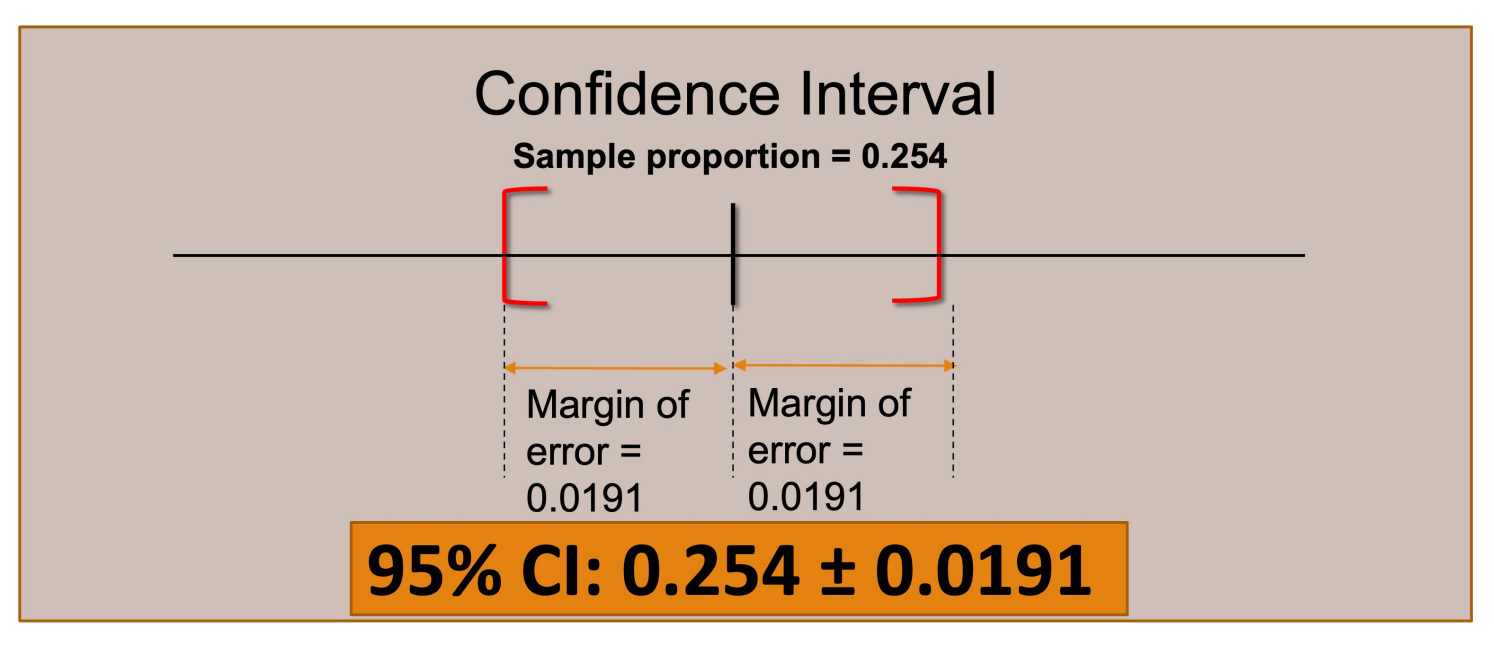
\includegraphics[width=0.6\linewidth]{images/chapter4-confidence-interval-proportion-example.png}
    \caption{Confidence Interval on Population Proportion Example}
    \label{fig:confidence-interval-proportion-example}
\end{figure}
So, the interpretation we have may be as follows:
\begin{center}
    We are 95\% confident that the population proportion (the parameter in this case) lies within the confidence level.
\end{center}
Using the idea of repeated sampling \footnote{It means that many simple random samples of the same size are taken and with the different sample statistics obtained from the different samples, different confidence intervals are constructed using the same method as above.}, the interpretation of ``95\% confident'' is that if \textbf{many simple random samples of the same size are taken, and a confidence level is constructed for each of them}, then \textbf{about 95\% of the confidence intervals constructed would contain the population parameter}.

This means if we collected 100 simple random samples and their 95\% confidence intervals were computed in the same manner, then about 95 out of 100 confidence intervals will contain the population parameter.
\begin{notebox}
    \begin{remark}
        It is wrong to say that there is a 95\% chance that the population parameter is \textbf{in the interval} (and 5\% chance that it is not)! The element of chance (or probability) comes from the \textbf{uncertainty of sampling} rather than the \textbf{uncertainty in the value of the population parameter}, whereas the latter is always fixed!
    \end{remark}
\end{notebox}
\textbf{Properties of Confidence intervals}
\begin{enumerate}
    \item The larger the sample size $n$, the smaller the random error (a.k.a margin error).
    \item The higher the confidence level at which the confidence interval is constructed (a.k.a the larger the $z^*$), the wider the confidence interval.
\end{enumerate}
\subsubsection{Confidence Interval for population mean}
The formula we use is
\begin{equation}
    \bar{x}\pm t^*\times \frac{s}{\sqrt{n}}
\end{equation}
where
\begin{align*}
    \bar{x}&=\text{sample mean} \\
    t^*&=\text{``t-value'' from t-distribution}\\
    s&=\text{sample standard deviation}\\
    n&=\text{sample size}
\end{align*}
\begin{notebox}
    \begin{remark}
        The exact value of $t^*$ depends on the sample size $n$ and the confidence level of the confidence interval we are constructing. Again, this is chosen by the software.
    \end{remark}
\end{notebox}
For example, let's suppose the confidence interval for the population mean we found to be $448727\pm6706.01$, we can similarly get an illustrative graph as follows,
\begin{figure}[H]
    \centering
    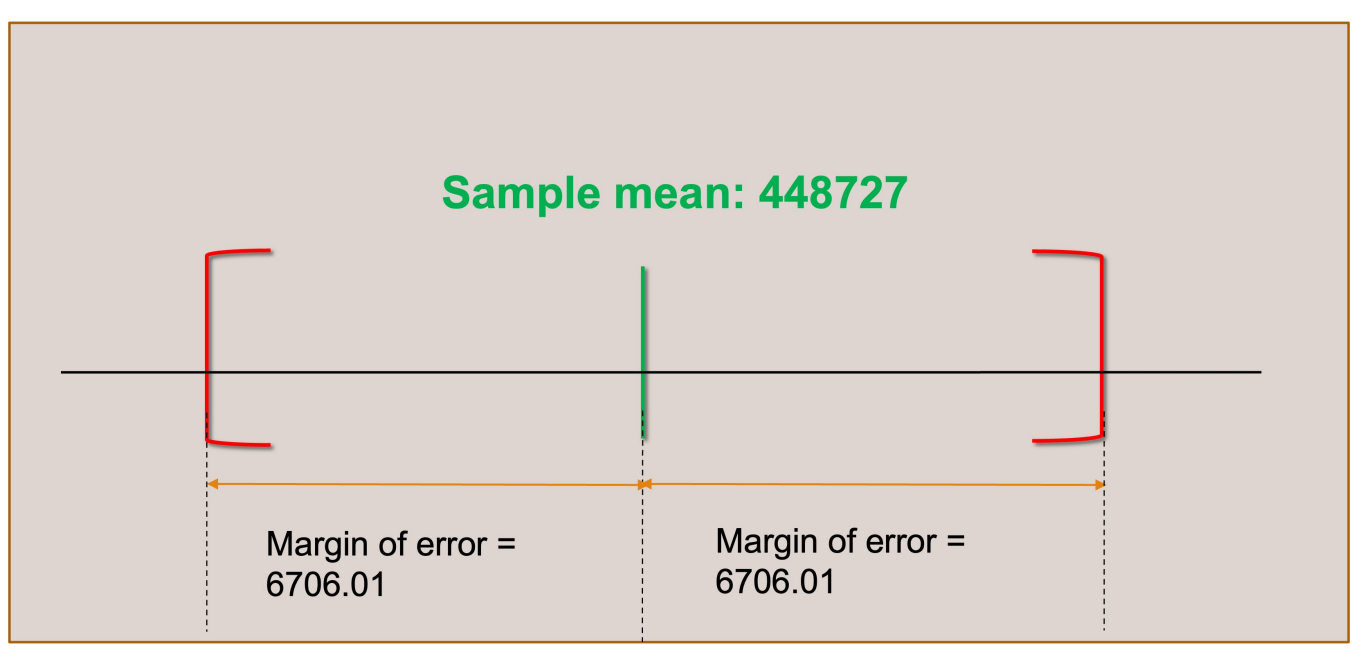
\includegraphics[width=0.5\linewidth]{images/chapter4-confidence-interval-population-mean-example.png}
    \caption{Confidence Interval on Population Mean Example}
    \label{fig:confidence-interval-population-mean-example}
\end{figure}

\subsection{Hypothesis Testing}
In statistics, when we want to test an idea or make a decision about something (like whether a new drug works or if a coin is fair), we use a method called \textbf{hypothesis testing}. This involves setting up two competing statements: the \textbf{null hypothesis} and the \textbf{alternative hypothesis}.
\begin{dfnbox}{Hypothesis Test}{dfn-hypothesis-test}
    A {\color{red} \textbf{hypothesis test}} is a statistical inference method used to decide if the data from a random sample is \textbf{sufficient} to support a particular hypothesis about a population.
\end{dfnbox}
In this course, we will focus on two types of hypothesis about the population, in particular, whether,
\begin{enumerate}
    \item a population parameter is $x$;
    \item in the population, 2 categorical variables $A$ and $B$ are associated with each other.
\end{enumerate}
\begin{dfnbox}{Null Hypothesis}{dfn-null-hypothesis}
    {\color{red} \textbf{Null hypothesis $H_0$}} is the default assumption. 
    \begin{enumerate}
        \item In case 1\footnote{population parameter is x}, it says there’s \textbf{no effect, no difference}, or that things are equal to a specific value.\footnote{Think of it as the ``nothing special is happening'' statement.} We assume it’s true unless we find strong evidence against it.
        \item In case 2\footnote{association between two categorical variables}, it means there is \textbf{no association}\footnote{Independence} between the two categorical variables.
    \end{enumerate}
\end{dfnbox}
\begin{dfnbox}{Alternative Hypothesis}{dfn-alternative-hypothesis}
    {\color{red} \textbf{Alternative Hypothesis $H_1$}} is the opposite — it’s what we’re trying to find evidence for.
    \begin{enumerate}
        \item In case 1, it says there is \textbf{an effect, a difference}, or that something doesn’t equal a specific value.\footnote{It’s the ``something interesting is happening'' statement.}
        \item In case 2, it means there is \textbf{an association}\footnote{Dependence} between the two categorical variables.
    \end{enumerate}
\end{dfnbox}
\begin{notebox}
    \begin{remark}
        The \textbf{null} and \textbf{alternative} hypotheses should be mutually exclusive, meaning that they \textbf{cannot be true simultaneously}.
    \end{remark}
\end{notebox}
Imagine you’re testing a new teaching method to see if it improves students’ test scores compared to the old method.
\begin{itemize}
    \item \textbf{Null Hypothesis} ($H_0$): The new teaching method doesn’t make a difference—the average test scores are the same as with the old method.
    \item \textbf{Alternative Hypothesis} ($H_1$): The new teaching method does make a difference—the average test scores are higher (or different) with the new method.
\end{itemize}
\subsubsection{Five steps for hypothesis testing}
\begin{enumerate}
    \item Identify \textbf{the question and state the \textit{null hypothesis} and \textit{alternative hypothesis}}.\footnote{How these hypotheses are stated depends on the context of the question and our aim.}
    \item Set the \textbf{\textit{significance level}} of our test.\footnote{For this course, you just need to know it's about choosing a number.}
    \item Using our sample, we find the relevant sample statistic.\footnote{This means calculating the population parameter we want but using the sample data. In \textbf{association tests}, this means we assume the null hypothesis is true and recalculate the corresponding data.}
    \item With the sample statistic and the hypothesis, we can calculate the $p$-value.\footnote{This is usually done by the software.}
    \item Make a conclusion of the hypothesis test.\footnote{What the conclusion turns out to be depends on the $p$-value calculated and the significance level set for the test.}
    \begin{enumerate}
        \item If the p-value is \textbf{smaller than} the significance level, you \textbf{reject the null hypothesis} and say there is evidence for the alternative hypothesis.
        \item Otherwise, you \textbf{fail to reject the null hypothesis}, meaning you don’t have enough evidence to support the alternative.
        \begin{notebox}
            Note: You don’t “accept” the null, you just don’t have proof against it.
        \end{notebox}
    \end{enumerate}
\end{enumerate}
\begin{dfnbox}{$p$-value}{dfn-p-value}
    The {\color{red} \textbf{$p$-value}} is the probability of obtaining a result \textbf{as extreme} or \textbf{more extreme} than our observation in the direction of the alternative hypothesis, \textbf{assuming the null hypothesis is true}.
\end{dfnbox}
\begin{notebox}
    \begin{remark}
        This $p$-value is usually calculated by the software.
    \end{remark}
\end{notebox}

\end{document}
